\documentclass[12pt]{book}

\usepackage[margin=0.8in]{geometry}
\usepackage[utf8]{inputenc}
\usepackage{hyperref}
\usepackage{graphicx}
\usepackage{amsmath}
\usepackage{pgfplots}
\usepackage{xcolor}
\usepackage{listings}
\usepackage{amssymb}
\usepackage{float}

\usepackage{fancyhdr}


\lstset{language=[90]Fortran,
  basicstyle=\ttfamily,
  keywordstyle=\color[HTML]{B22222},
  commentstyle=\color[HTML]{555555},
  morecomment=[l]{!\ }% Comment only with space after !
}

\pgfplotsset{width=10cm,compat=1.9}
\graphicspath{{./img}}

\usepgfplotslibrary{external}
\usetikzlibrary{calc}

\let\cleardoublepage=\clearpage

\newcommand\Chapter[2]{
  \chapter[#1: {\itshape#2}]{#1\\[2ex]\Large\itshape#2}
}

\newcommand{\changefont}{
    \fontsize{9}{11}\selectfont
}
\fancyhf{}

\fancyhead[L]{\changefont \slshape \leftmark\\}
\fancyhead[R]{\changefont \slshape \rightmark}
\fancyfoot[R]{\thepage}
\pagestyle{fancy}

\title{\textbf{Artificial neurons notes}\\
  \vspace{1cm} % Adjust the value to increase or decrease the vertical space
  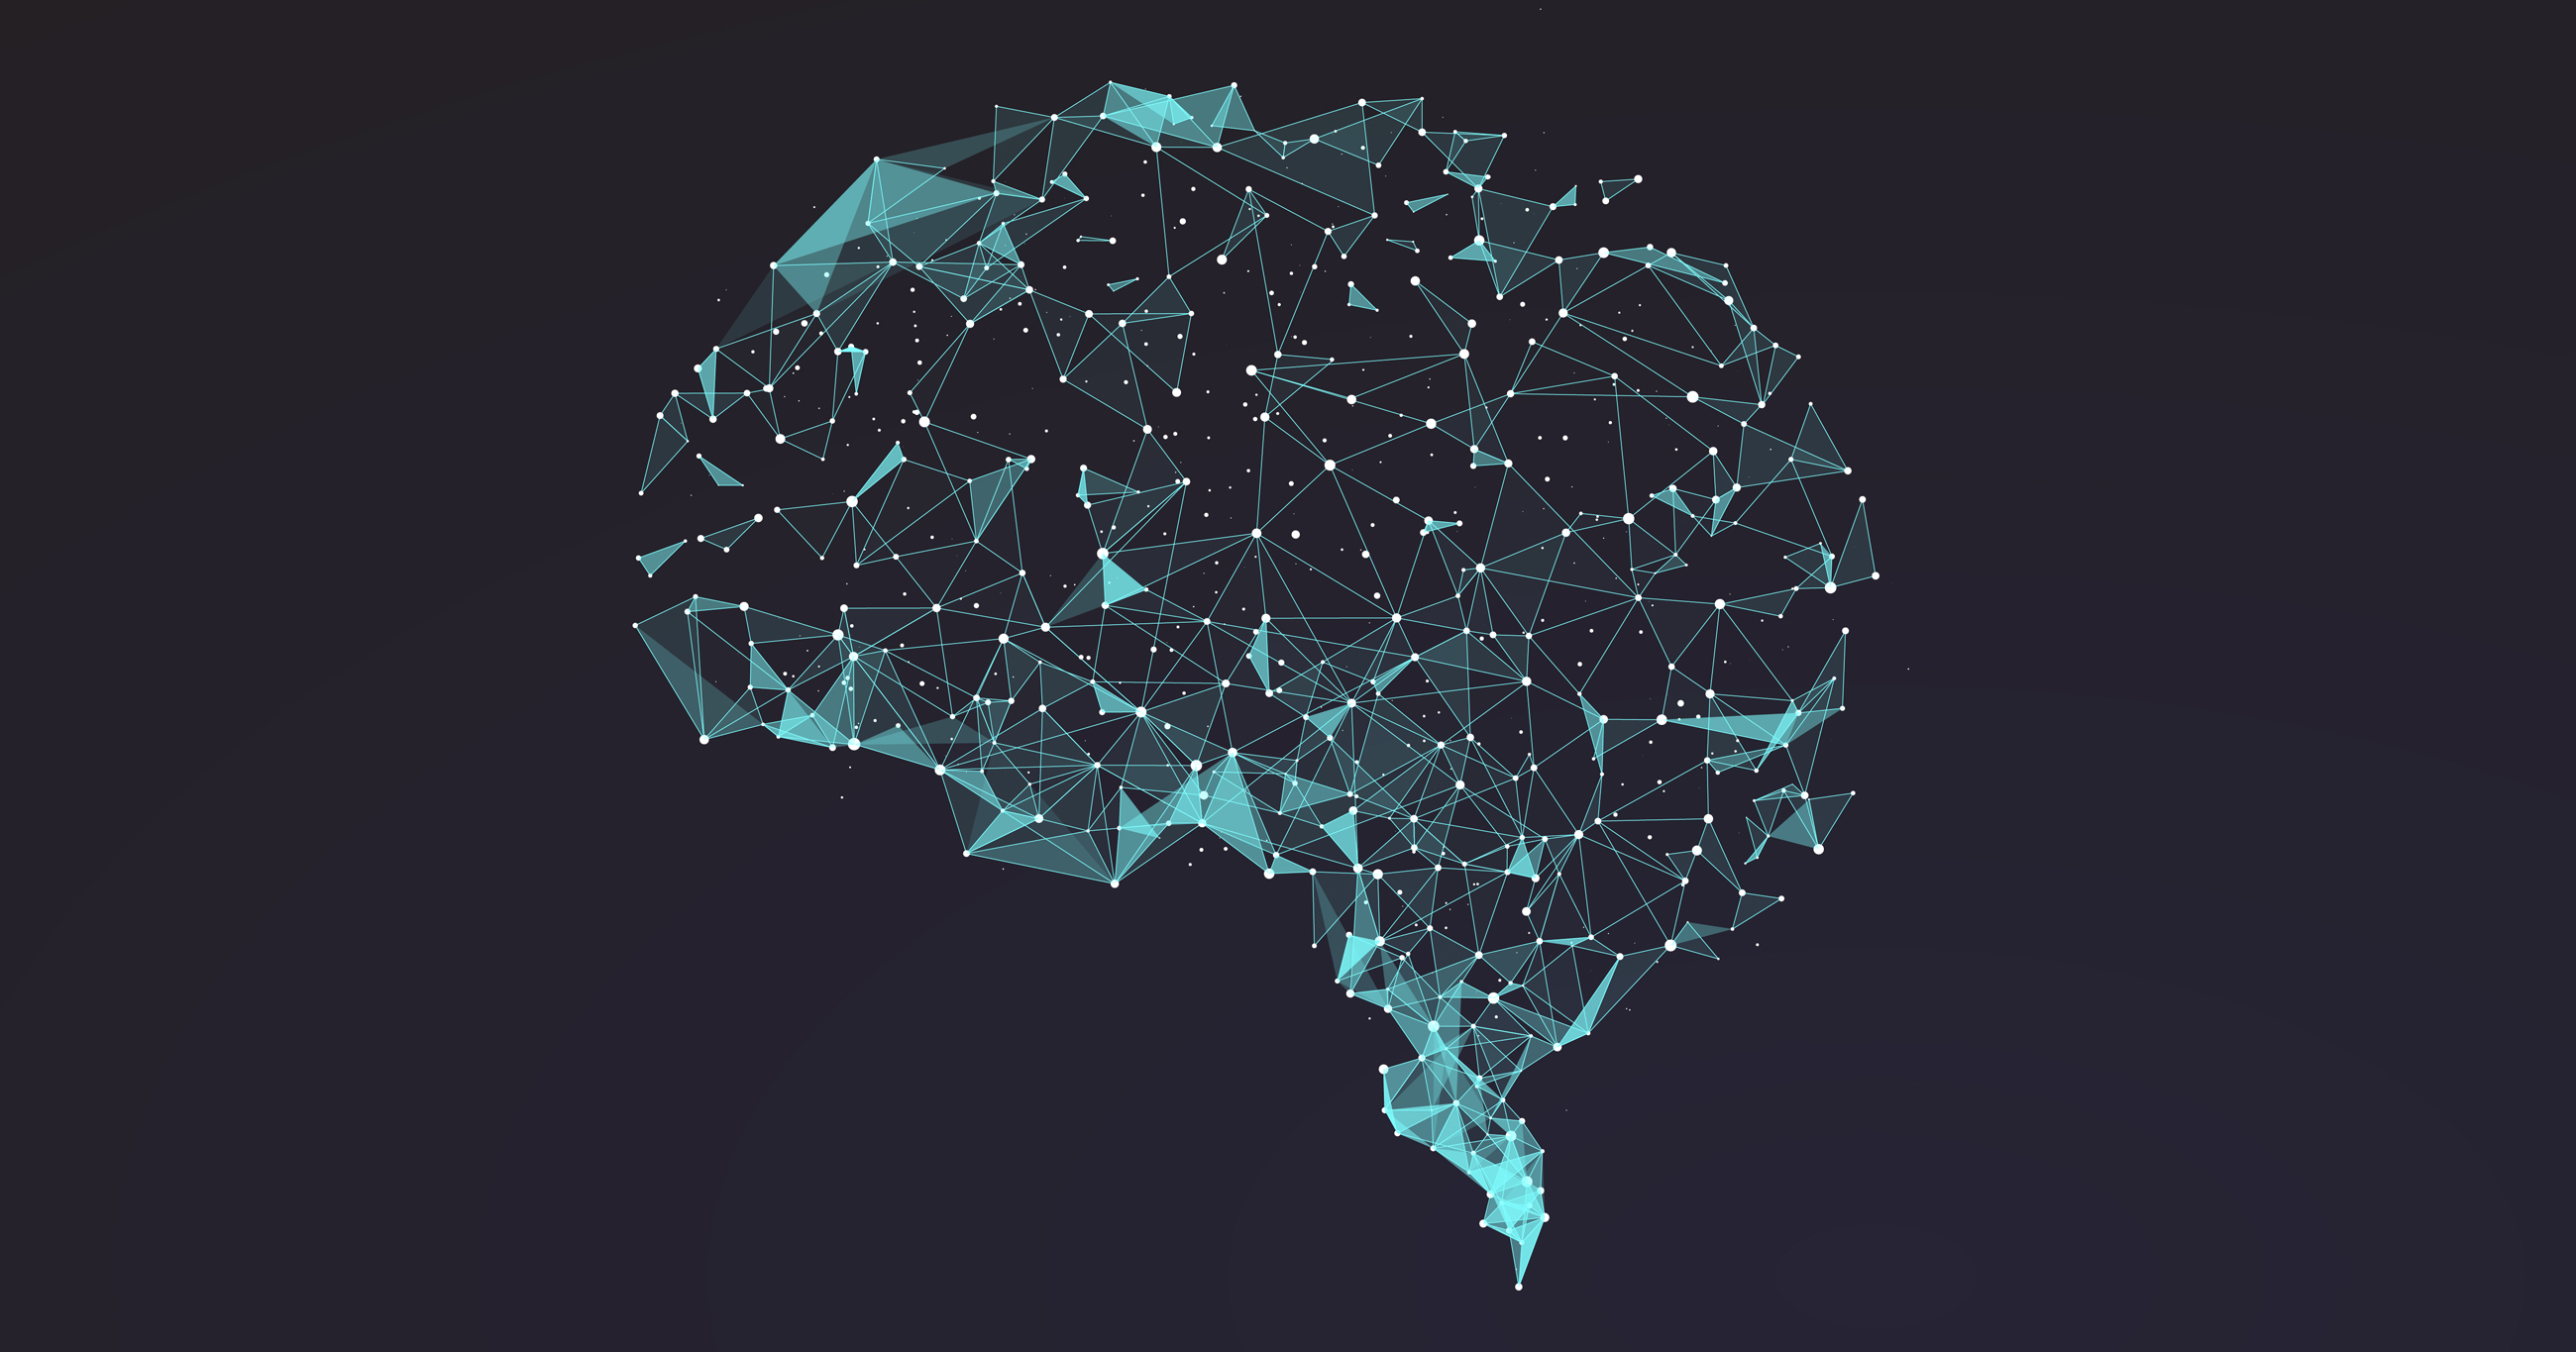
\includegraphics[scale = 0.7]{cover_page.jpg}
}
\author{By \textbf{Erick Alejandro Carrillo López}.}
\date{2023/04/03}

\begin{document}
\maketitle

\tableofcontents
\addcontentsline{toc}{chapter}{Table of contents}

\Chapter{Introduction}{The purpuse of these notes}


\section{About these notes}
This is just my personal compilation of notes. The purpose of this document is not professional;
it is simply a recompilation of my studies on artificial intelligence and its algorithms from scratch.

I have gathered information from various sources and documented my understanding, insights, and observations
on the subject matter. It serves as a reference and a way for me to solidify my knowledge.

Throughout this document, I aim to explore the fundamental concepts, theories, and techniques in the field
of artificial intelligence. From machine learning algorithms to neural networks, I delve into the intricacies
of these topics, providing explanations and examples along the way.

Please note that the information presented here is based on my personal interpretation and may not encompass
the entirety of the subject. Therefore, it is always recommended to refer to authoritative sources for a
comprehensive understanding of artificial intelligence.

I hope this document proves to be a valuable resource for those interested in learning about artificial
intelligence, as well as a testament to my own growth and development in this fascinating field.




\Chapter{What is an artificial neuron?}{The perceptron and its proof of convergence}

\section{What is it?}
\subsection{A real neuron}
A real neuron, also known as a nerve cell, is a specialized cell that transmits
electrical and chemical signals in the nervous system.\\
At the most basic level, a neuron consists of a cell body, dendrites, and an axon.
The cell body contains the nucleus and other organelles, and serves as the metabolic center
of the neuron. Dendrites are thin, branching extensions that receive signals from other
neurons or sensory cells. The axon is a long, thin projection that carries signals away
from the cell body to other neurons or target cells.
\begin{figure}[h]
  \centering
  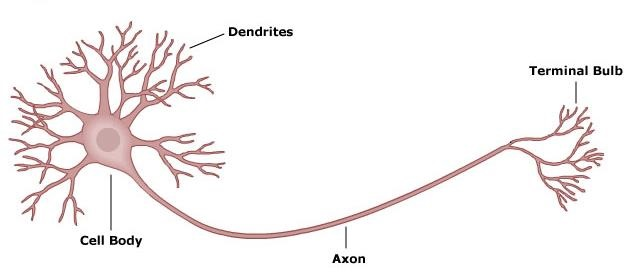
\includegraphics[scale = 0.5]{cell-body.jpg}
  \caption{Cell Body with its axon}
\end{figure}
Neurons communicate with each other through synapses, which are specialized
junctions between neurons. When an electrical signal, known as an action potential,
reaches the end of an axon, it triggers the release of neurotransmitter molecules, which diffuse
across the synapse and bind to receptors on the dendrites or cell body of the target neuron. This
binding can cause the target neuron to generate its own action potential, which propagates down its
axon to signal other neurons or target cells.
\begin{figure}[h]
  \centering
  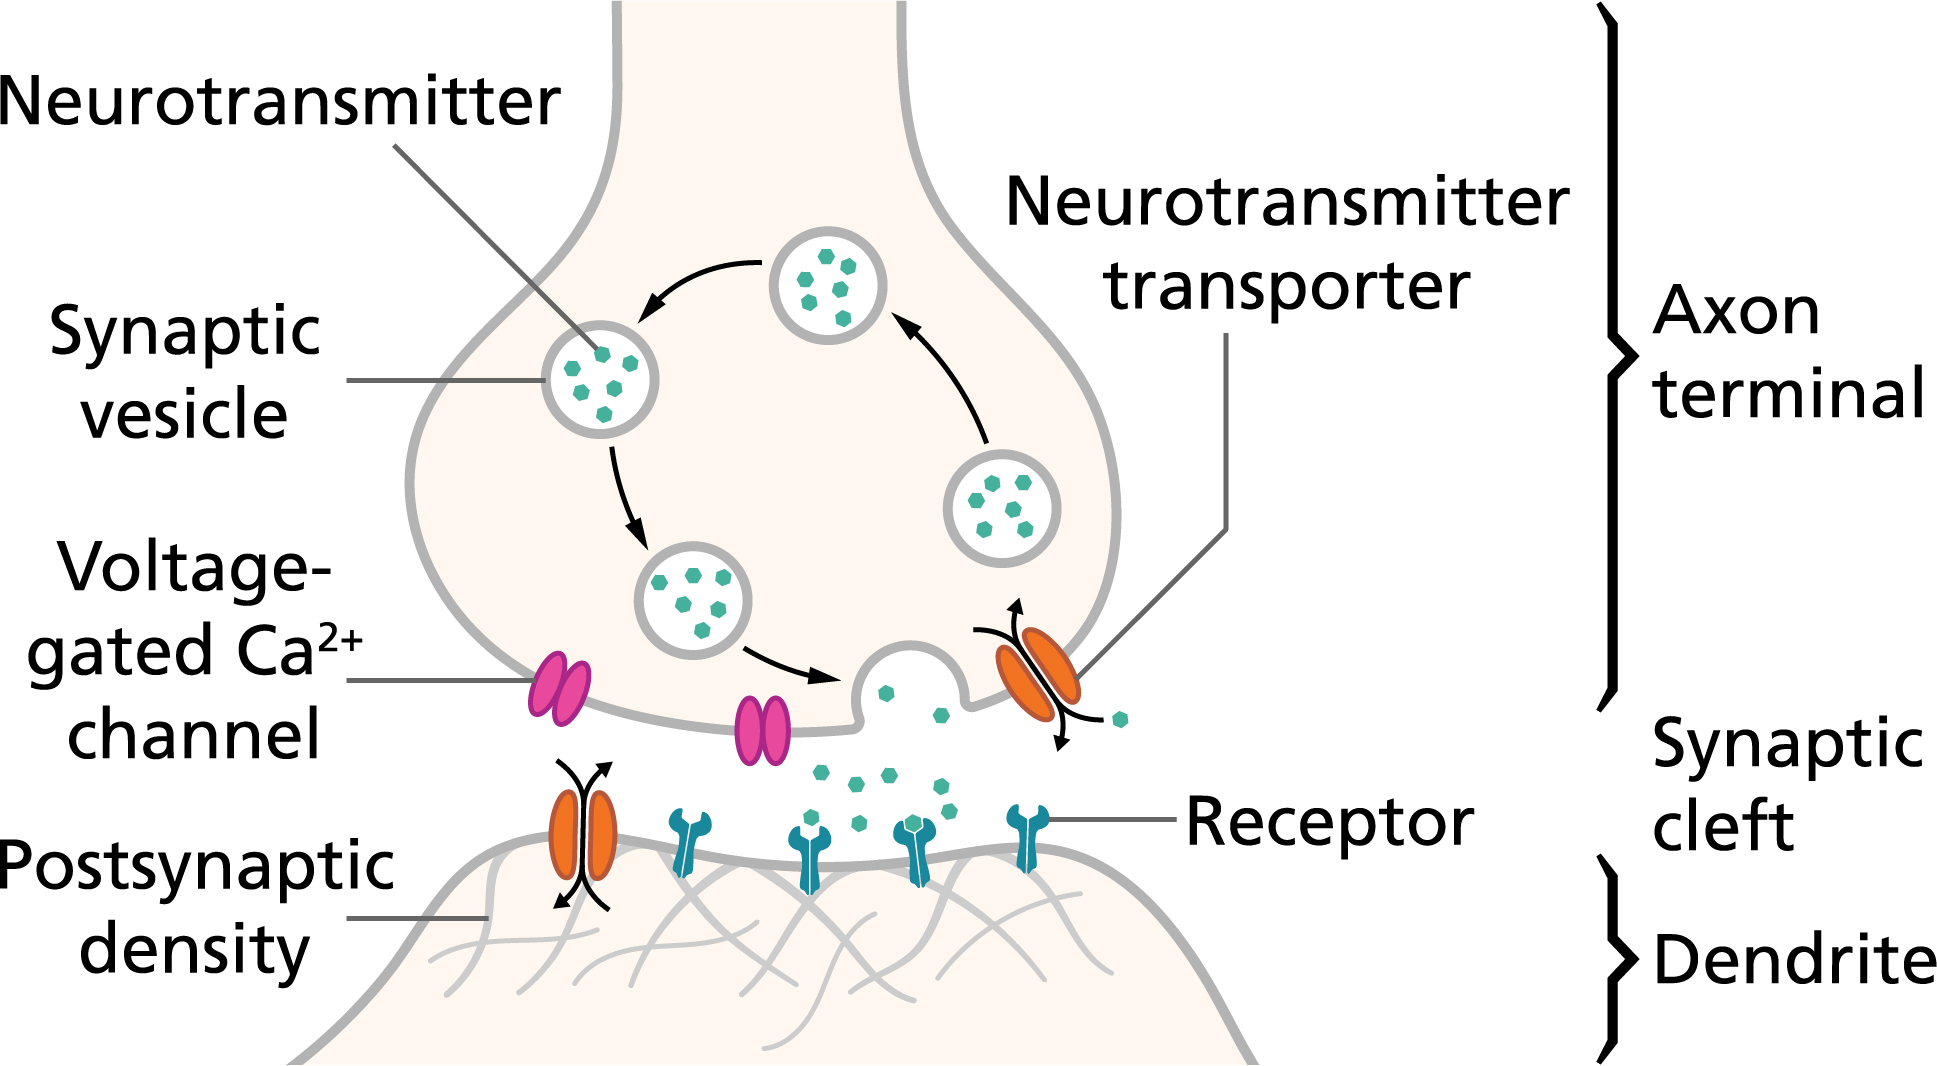
\includegraphics[scale = 0.19]{Synapse.jpg}
  \caption{Synapse}
\end{figure}

Neurons talk to each other across synapses. When an action potential reaches the
presynaptic terminal, it causes neurotransmitter to be released from the neuron into the synaptic
cleft, a 20–40nm gap between the presynaptic axon terminal and the postsynaptic dendrite
(often a spine).\\
After travelling across the synaptic cleft, the transmitter will attach to neurotransmitter
receptors on the postsynaptic side, and depending on the neurotransmitter released
(which is dependent on the type of neuron releasing it), particular positive (e.g. Na+, K+, Ca+)
or negative ions (e.g. Cl-) will travel through channels that span the membrane.
\subsection{The perceptron}
The perceptron is a type of artificial neural network that is loosely modeled after the structure
and function of real neurons in the brain. The basic idea behind the perceptron is to use a
mathematical algorithm to simulate the behavior of a simplified neuron, which can then be used to
perform simple classification tasks.\\
The perceptron consists of an input layer, a set of weights, a summing or activation function,
and an output.
The input layer consists of one or more nodes, each of which represents a feature of the input data.
The weights are values that are assigned to each input node, which control the strength of the
connection between that node and the output.
\begin{figure}[h]
  \centering
  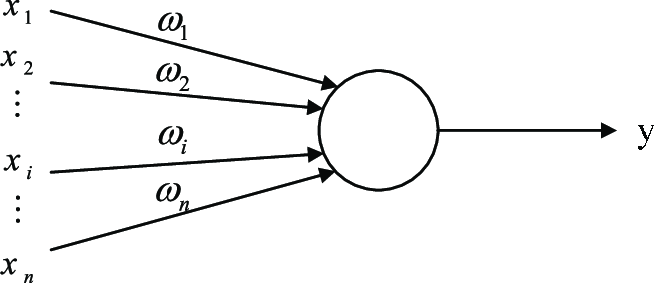
\includegraphics[scale = 0.5]{perceptron.png}
  \caption{Perceptron}
\end{figure}

The summing or activation function takes the weighted inputs and adds them together to produce a
single output
value. This output value is then compared to a threshold value, which determines whether the
perceptron will output a positive or negative value. If the output is positive, the perceptron
classifies the input as belonging to one class; if it is negative, the input is classified as
belonging to the other class.
\subsection{Perceptron parts}
\begin{itemize}
\item \textbf{Input Nodes or Input Layer:} \\
  This is the primary component of Perceptron which accepts the initial data into the system for
  further processing. Each input node contains a real numerical value.
\item \textbf{Wight and Bias:} \\
  Weight parameter represents the strength of the connection between units. This is another most
  important parameter of Perceptron components. Weight is directly proportional to the strength of the
  associated input neuron in deciding the output. Further, Bias can be considered as the line of
  intercept in a linear equation.
\item \textbf{Activation Function:} \\
  These are the final and important components that help to determine whether the neuron will
  fire or not. Activation Function can be considered primarily as a step function.\\
  \textbf{Types of Activation functions:}
  \begin{itemize}
  \item Sign function.
  \item Step function.
  \item Sigmoid function.
  \end{itemize}
  \begin{figure}[h]
    \centering
    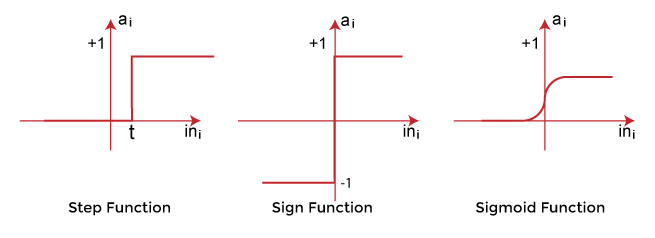
\includegraphics[scale = 0.5]{funcs.png}
    \caption{Types of activation functions}
  \end{figure}
\end{itemize}
\section{Códing the perceptron}
\subsection{The Perceptron Algorithm}
Perceptron model works in two important steps as follows.
\begin{enumerate}
\item In the first step first, multiply all input values with corresponding weight values and then add
  them to determine the weighted sum. Mathematically, we can calculate the weighted sum as follows.\\
  \[
    \sum_{i = 0}^{n}(weight_i \cdot input_i) = \sum_{i = 0}^{n}(w_i \cdot x_i) = w_0 \cdot x_0 + w_1 \cdot x_1
    + \cdots + w_n \cdot x_n
  \]\\
  Add a special term called bias 'b' to this weighted sum to improve the model's performance.\\
  \[
    \sum_{i = 0}^{n}(w_i \cdot x_i) + b
  \]
\item In the second step, an activation function is applied with the above-mentioned weighted sum,
  which gives us output either in binary form or a continuous value as follows.\\
  \[
    y = activation(\sum_{i = 0}^{n}(w_i \cdot x_i) + b) = activation(\vec{w} \cdot \vec{x} + b)
  \]
\end{enumerate}
At the end what we are doing here is a simple dot product of two vectors, put it in the activation
function.
\[
  \sum_{i = 0}^{n}(w_i \cdot x_i) + b = \vec{w} \cdot \vec{x} 
\]
Where.
\[
  \vec{w} = (b, w_1, \cdots, w_n)
\]
\[
  w_0 = b
\]
\[
  \vec{x} = (1, x_1, \cdots, x_n)
\]
\[
  x_0 = 1
\]
We can think of this as a hyperplane for each component $\forall x$ and the result of the dot product.

\begin{figure}[!hb]
  \centering
  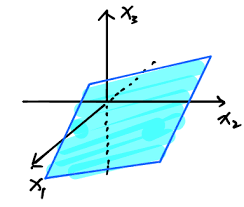
\includegraphics[scale = 1]{plane.png}
  \caption{A hyperplane}
\end{figure}

\subsection{From the perceptron algorithm to code}
Firstly declare the threshold variable or bias variable,
this variable will be used as a threshold or bias for the activation function.
\begin{verbatim}
const threshold = 1.5
\end{verbatim}
After that declare two arrays the weights and input, the weights array is always initialized with random
values.
\begin{verbatim}
input = [1, 0, 1, 0, 1]
weights = [0.7, 0.6, 0.5, 0.3, 0.4]
\end{verbatim}
The weighted sum of the input values and weights by initializing a variable called sum to zero,
and then iterating over the input values and weights and adding the product of each input value
and weight to sum.
\begin{verbatim}
sum = 0.0
for (i = 0, i < input.length, i++)
    sum += input[i] * weights[i]
\end{verbatim}
And at the end just apply an activation function, a sign function to the weighted sum by checking
if sum is greater
than the threshold value of 1.5. If sum is greater than 1.5,
the activate variable is set to 1, otherwise, it is set to -1.
\begin{verbatim}
activate = (sum > threshold) ? 1 : -1
\end{verbatim}
Overall, this code represents a simple example of how a perceptron might work by calculating a
weighted sum of inputs and weights and applying a threshold activation function to produce a
binary output.
\subsection{The perceptron learning algorithm}
To train a perceptron, we need to adjust the weights of the input connections so that the perceptron produces
the desired output for a given set of inputs. This is achieved through an iterative algorithm called the
perceptron learning algorithm.

The core concept behind the perceptron learning algorithm is to utilize the error and
desired outputs to modify the weights, thus improving the perceptron's ability to generate the desired output.

It is important to note that the perceptron learning algorithm assumes the problem to be linearly separable,
meaning that there exists a hyperplane capable of separating the examples in two spaces.
If the problem is not linearly separable, the perceptron may fail to converge to a solution.

In simpler terms, the perceptron learning process can be summarized in these three steps:
\begin{enumerate}
\item The training function makes predictions based on the activation function, which can be represented
  as $f(\vec{x}_t) = \vec{x}_t \cdot \vec{w}_k$, where $t$ denotes the current iteration through the training
  data, and $k$ represents the current state of the weights.

\item If the guess is incorrect, the perceptron adjusts the weights. There are different ways to perform this
  adjustment, but one common approach is to utilize useful information such as the input vector $\vec{x}$,
  the desired output $y_t$, and a learning rate $\gamma$ (where $\gamma$ is a small value, $\gamma < 1$).
  The weight adjustment can be expressed as $\vec{w}_{k+1} = \vec{w}_k + \gamma y_t \vec{x}_t$.

\item After many guesses and adjustments, the weights will converge to the desired weights denoted as
  $\vec{\theta}^*$, which can be represented as
  $k \rightarrow \infty \quad \implies \quad \vec{w}_k \rightarrow \vec{\theta}^*$.
\end{enumerate}

By following these steps, the perceptron learns and adapts its weights until it achieves accurate
classifications.

\begin{figure}[h]
  \centering
  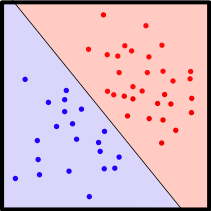
\includegraphics{linearly.png}
  \caption{Linear separability}
\end{figure}
\subsubsection{The Mathematical definition behind linear separability}
Let $X_0$ and $X_1$ be two sets of points in an n-dimensional Euclidean space. Then $X_0$ and $X_1$
are linearly separable, if there exist $n + 1$ real numbers $w_1, w_2, \cdots, w_n, k$ such that
every point $x \in X_0$ satisfies $\sum_{i = 1}^{n}(w_i \cdot x_i) > k$ and every point $x \in X_1$
satisfies
$\sum_{i = 0}^{n}(w_i \cdot x_i) < k$ where $x_i$ is the i-th component of $x$.
\subsection{From the learning algorithm to code}
You must create a training function with these characteristics using the previous three steps,
so define the activation function which at the end it is a simple binary function.
\begin{verbatim}
int activation(x)
    return (x > 0) ? 1 : -1
\end{verbatim}
Define the learning rate and a number of epochs, which is the amount of times that we are going
train the perceptron and the learning rate represents how fast our perceptron is going to learn.
\begin{verbatim}
learning_rate = 0.1
num_epochs = 100
\end{verbatim}
Train the perceptron by iterating with all the training data which in this case it is an bidimensinal
array and a simple threshold or bias.
\begin{verbatim}
for (i = 0, i < num_epochs, i++)
    for (j = 0, j < inputs.length, j++)
        sum = 0.0
        for (k = 0, k < weights.length, k++)
            sum += inputs[j][k] * weights[i]
        sum += b
        out = activation(sum)
\end{verbatim}
At the end, the adjustment of weights and bias is performed based on the error at the inputs within a loop.
The calculation of the error is a straightforward subtraction process. Subsequently, the error is utilized in
conjunction with the learning rate to update the weights and bias.
\begin{verbatim}
error = label[j] - output
for (k = 0, k < weights.length, k++)
    weights[k] += learning_rate * error * inputs[j][k]
b += learning_rate * error
\end{verbatim}
\section{The math behind of the learning algorithm}
Maybe now the main question is why we adjust the weights like that.
\begin{verbatim}
weights[k] += learning_rate * error * inputs[j][k]
\end{verbatim}
And the bias or threshold.
\begin{verbatim}
b += learning_rate * error
\end{verbatim}
To answer that we need to formulate a math function that represents our neuron which receives a vector
as input.
\[
  f(\vec{x}) = 
  \begin{cases}
    1 &\quad if \vec{w} \cdot \vec{x} > 0  \\
    -1 &\quad \text{otherwise} \\
  \end{cases}
\]

Where $\vec{w} = (b, w_1, \cdots, w_n)$
is the coefficients or weights, $\vec{x} = (1, x_1, \cdots, x_n)$
the input vector, so from this idea we can come up
with something like this.
\[
  y_t = 1 \implies \vec{w} \cdot \vec{x}_t > 0
\]

\[
  y_t =  - 1 \implies \vec{w} \cdot \vec{x}_t \le 0
\]
Where $(\vec{x}_t, y_t) \in \mathbb{D}$ which is the whole dataset, then from these implications
we can formulate two inequalities that
represent when the perceptron is wrong and when it is correct.
\[
  \text{Correct} \implies y_t \cdot \vec{x}_t \cdot \vec{w} > 0
\]

\[
  \text{Wrong} \implies y_t \cdot \vec{x}_t \cdot \vec{w} \le 0
\]

At the end what we want is a desired vector $\vec{\theta}^*$ which fulfills a single characteristic.
\[
  \exists \vec{\theta}^* \in \mathbb{R}^{d} \quad|\quad y_t\vec{\theta}^*\vec{x}_t > 0,\quad
  \forall (\vec{x}_t, y_t) \in \mathbb{D}
\]
Where $\vec{\theta}^*$ is the desired vector configuration which classifies the inputs perfectly
and $\mathbb{D}$ is the data set,
then when the perceptron gets an error this both inequalities are true.
\[
  y_t\vec{w}_k \vec{x} \le 0 \Leftrightarrow  y_t \not = y'
\]
Where $y'$ is the result obtained,
then in the algorithm when that happens we update the $\vec{w}$ like this.
\[
  \vec{w}_{k + 1} = \vec{w}_{k} + y_t\vec{x}_t
\]
In the algorithm we try to make those changes less aggressive, so to understand
why we adjust the weights like that, think on this chart.
\begin{center}
\begin{tikzpicture}[scale=1.5]
  \draw[thick,->] (2,0) -- (0,1) node[anchor=south west]{$\vec{w}_k$};
  \draw[thick,->] (2,0) -- (5,0) node[anchor=south west]{$\vec{\theta}^*$};
\end{tikzpicture}
\end{center}
Again the $\vec{\theta}^*$ is the desired vector configuration which for any
$(\vec{x}_t, y_t) \in \mathbb{D}$ returns an $y' = y_t$ and the $\vec{w}_k$ is the current k-th iteration
of the weights, obviously we don't know where $\vec{\theta}^*$ is, but we can approximate $\vec{w}_k$
to $\vec{\theta}^*$ by a 
simple additions of vectors,
then We can put the vector $y_t \cdot \vec{x}_t$ in the chart.
\begin{center}
\begin{tikzpicture}[scale=1.5]
  \draw[thick,->] (2,0) -- (0,1) node[anchor=south west]{$\vec{w}_k$};
  \draw[thick,->] (2,0) -- (5,0) node[anchor=south west]{$\vec{\theta}^*$};
  \draw[thick,->] (2,0) -- (5,-1) node[anchor=south west]{$y_t\vec{x}_t$};
\end{tikzpicture}
\end{center}
Then if we compute
the dot product of these two vectors $y_t\vec{x}_t \cdot \vec{\theta}^*$ this inequalitie
becomes true.
\[
  y_t\vec{\theta}^*\vec{x}_t > 0
\]
Because again the $\vec{\theta}^*$ is the desired vector configuration, the meaning of the dot product
of two vectors is how much they are pointing in the same direction,
if the dot product of two vectors is positive, it means they are pointing in
roughly the same direction, if it is negative, they are pointing in roughly opposite
directions, and if it is zero, they are perpendicular (at a right angle) to each other,
then the dot product of two Euclidean vectors $\vec{v}$ and $\vec{u}$ is defined by.
\[
  \vec{v} \cdot \vec{u} = ||\vec{v}|| \cdot ||\vec{u}|| \cdot \cos{\theta}
\]
Where $\theta$ is the angle between $\vec{v}$ and $\vec{u}$, so
from that idea we can perfectly infer that $y_t\vec{x}_t \cdot \vec{w}_k \le 0$ by their angle.\\
\begin{center}
\begin{tikzpicture}[scale=1.5]
  \draw[thick,->] (2,0) -- (0,1) node[anchor=south west]{$\vec{w}_k$};
  \draw[thick,->] (2,0) -- (5,0) node[anchor=south west]{$\vec{\theta}^*$};
  \draw[thick,->] (2,0) -- (5,-1) node[anchor=south west]{$y_t\vec{x}_t$};

  \draw let \p1 = (-2,1), \p2 = (5,-1.78), \n1 = {atan2(\y1,\x1)}, \n2 = {atan2(\y2,\x2)} in (2,0) + (\n1:0.8) arc (\n1:\n2:0.8) node[midway, above right] {$\theta$};
\end{tikzpicture} \\
\end{center}
So think in the addition of vector as way to rotate a vector, look if I sum $\vec{w}_k + y_t\vec{x}_t$
I get the next iteration the $k + 1$ iteration which results on this new vector $\vec{w}_{k + 1}$.
\begin{center}
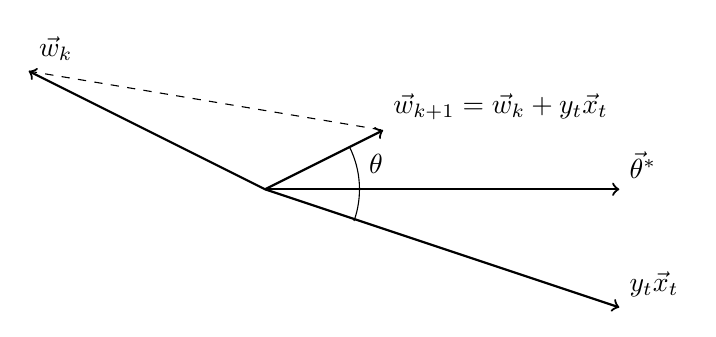
\begin{tikzpicture}[scale=1.5]
  \draw[thick,->] (2,0) -- (0,1) node[anchor=south west]{$\vec{w}_k$};
  \draw[thick,->] (2,0) -- (5,0) node[anchor=south west]{$\vec{\theta}^*$};
  \draw[thick,->] (2,0) -- (5,-1) node[anchor=south west]{$y_t\vec{x}_t$};
  \draw[thick,->] (2,0) -- (3,0.5) node[anchor=south west]{$\vec{w}_{k + 1} = \vec{w}_k + y_t\vec{x}_t$};
  \draw[dashed] (0,1) -- (3,0.5);
  
  \draw let \p1 = (2,1), \p2 = (5,-1.78), \n1 = {atan2(\y1,\x1)}, \n2 = {atan2(\y2,\x2)} in (2,0) + (\n1:0.8) arc (\n1:\n2:0.8) node[midway, above right] {$\theta$};
\end{tikzpicture} \\
\end{center}
With this new vector $\vec{w}_{k+1}$ we generate a new angle $\theta$ that makes
this inequalitie $\vec{w}_{k+1} \cdot y_t\vec{x}_t \le 0$
false 
which implies that the perceptron have learned the pattern, basically we adjust the weights
 to new direction.
\[
  \neg (\vec{w}_{k+1} \cdot y_t\vec{x}_t \le 0) \implies \vec{w}_{k+1} \cdot y_t\vec{x}_t > 0\quad |
  \quad y' = y_t, \quad \vec{w}_k \rightarrow \vec{\theta}^*
\]
We are arriving to a conjecture which is that it looks like we need a finite amount of $k$
iterations to perfectly separate the points or vectors $\vec{x}_t$ in $\mathbb{D}$
making $\vec{w}_k \rightarrow \vec{\theta}^*$, creating that perfectly
hyperplane that separates the points.
This is so important because if that amount of iterations is infinite then the
algorithm is useless because means that we are not going to have any chance to classifie most of
the possible inputs,
but if it is a finite amount of iterations means that we are going to have the chance to
classifie most of the posible inputs
making this useful,  spoiler, there are finite amounts of iterations for a separable finite
set of tuples $(\vec{x}_t, y_t) \in \mathbb{D}$, so lets proof that.
\subsection{Perceptron Convergence Proof}
\label{sec:perceptron-convergence-proof}
Lets think in that variable $k$ which represents the amount of iterations,
It should be a finite real number.
\[
  k \in \mathbb{R}
\]
Then before to continue with the proof we need to do an assumption,
we are going to scale our $\vec{\theta}^*$ in another words we are going to change it
for an easy manipulation,
so for this section we are going to work with a new vector.
\[
  \vec{\theta}^* = \alpha \cdot \vec{\theta}\quad |\quad ||\vec{\theta}|| = 1
\]
So we scale the desired vector $\vec{\theta}^*$ for getting its unitary vector $\vec{\theta}$,
At the end the inequality is still being true.
\[
  y_t\vec{\theta}^*\vec{x}_t > 0
\]
\[
  y_t\alpha\cdot\vec{\theta}\vec{x}_t > 0
\]
\[
  \frac{1}{\alpha} \cdot y_t\alpha\vec{\theta}\vec{x}_t > 0 \cdot \frac{1}{\alpha}
\]
\[
  y_t\vec{\theta}\vec{x}_t > 0
\]
Obviously all the computed values with this new vector $\vec{\theta}$ are going to be lesser than
the comptued values with $\vec{\theta}^*$, to be exact is going to be $\alpha$ times greater, and
actually if you think we don't care how big these outputs are, we only care
that they are big enoguh to make that statement true the whole time.
\[
  y_t\vec{\theta}^*\vec{x}_t > y_t\vec{\theta}\vec{x}_t > 0
\]

To just finished with this idea think on this statement
and lets continue with the proof of the convergence.
\[
  \exists \vec{\theta}^* = \alpha \cdot \vec{\theta}\quad|\quad
  y_t\vec{\theta}^*\vec{x}_t > 0 \wedge
  y_t\vec{\theta}\vec{x}_t > 0,
  \quad \forall(\vec{x}_t, y_t)
  \in \mathbb{D}
\]

Then we need to think in this
dot product $\vec{w}_{k + 1} \cdot \vec{\theta}$ because this dot product
will grow but it will never decrease and why is that?, well because of the algorithm we only
rotate or adjust $\vec{w}_{k}$ when $\vec{w}_k \cdot \vec{x}_ty_t \le 0$, look this chart.
\begin{center}
\begin{tikzpicture}[scale = 0.8]
  \draw[->, thick] (-5,0)--(5,0) node[right]{$t$};
  \draw[->, thick] (0,-5)--(0,5) node[above]{$\vec{w}_{k + 1} \cdot \vec{\theta}$};
  
  \draw[black, thick] (0, -2) -- (0, -1) -- (0.5,-0.5) -- (1,0) -- (1.5, 1.5) -- (2, 2) -- (2.5, 3) -- (3, 3.5) -- (4, 3.5) -- (5, 5);
\end{tikzpicture}
\end{center}
You can imagine something like this, it never decreases, so why this dot product is useful?, well
because this dot product represents how the weights are being adjust or how the perceptron learns,
it would start in some negative real number but it will finish in some positive value,
and as I said before there is going to be a moment where $\vec{w}_{k+1} \cdot \vec{\theta}$
will never increase
anymore, at the end we would find inserting how this dot product grows through
the instances of $(\vec{x}_t, y_t)$.
\begin{center}
\begin{tikzpicture}[scale = 0.8]
  \draw[->, thick] (-5,0)--(10,0) node[right]{$t$};
  \draw[->, thick] (0,-5)--(0,5) node[above]{$\vec{w}_{k + 1} \cdot \vec{\theta}$};
  
  \draw[black, thick] (0, -2) -- (0, -1) -- (0.5,-0.5) -- (1,0) -- (1.5, 1.5) -- (2, 2) -- (2.5, 3) -- (3, 3.5) -- (4, 3.5) -- (5, 5) -- (10, 5);
\end{tikzpicture}
\end{center}
Let's imagine that we already have made a some $k$ iteration,
then we want to know what would be 
the minimum difference between this $k$ iterations $\vec{w}_{k+1} \cdot \vec{\theta}$ with It's
previous iteration $\vec{w}_{k} \cdot \vec{\theta}$, well.
\[
  \vec{w}_{k + 1} \cdot \vec{\theta} = (\vec{w}_{k} + y_t\vec{x}_t) \vec{\theta}
  = \vec{w}_{k}\vec{\theta} + y_t\vec{x}_t\vec{\theta}
\]
\[
  \vec{w}_{k + 1} \cdot \vec{\theta} -  \vec{w}_{k}\vec{\theta}
  =  y_t\vec{x}_t\vec{\theta}
\]
So basically this is
the difference $y_t\vec{x}_t\vec{\theta}$ which is $y_t\vec{x}_t\vec{\theta} > 0$ and so
from this expression we can create constant gamma which represents the minimum
difference of some pair of values $\vec{w}_{k+t} \cdot \vec{\theta} - \vec{w}_{k} \cdot \vec{\theta}$
by any $k$ iteration.
\[
  \gamma = minimum(y_t \vec{x}_t\vec{\theta}) \quad|\quad \forall (\vec{x}_t, y_t) \in \mathbb{D}
\]
We know that $y_t \in \{1, -1\}$, so we can forget it and use a simple absolute value.
\[
  \gamma = minimum(|\vec{x}_t\vec{\theta}|) \quad|\quad \forall (\vec{x}_t, y_t) \in \mathbb{D}
\]
\[
  |\vec{w}_{k + 1} \cdot \vec{\theta} -  \vec{w}_{k}\vec{\theta}|
  \ge \gamma\quad | \quad \forall \vec{w}_{k+1}
\]

Finally we can abstract this idea of $\gamma$ to an inequalitie for all the $k$ iterations.
\[
  \gamma \cdot k \le |\vec{w}_{k+1} \cdot \vec{\theta}| \le ||\vec{w}_{k+1}||\cdot ||\vec{\theta}||
  = ||\vec{w}_{k+1}||\quad|\quad \forall \vec{w}_{k + 1}
\]
\[
  \gamma \cdot k \le ||\vec{w}_{k+1}||\quad|\quad \forall \vec{w}_{k + 1}
\]
As you can see we replace $||\vec{\theta}|| = 1$, because if unitary vector and
$\gamma \cdot k$ works as lower bound for any $|\vec{w}_{k + 1}\cdot \vec{\theta} |$, this lead us
to think if there exist a higher bound, spoiler, It exists, to find it now we need to think in another
dot product which is this.
\[
  \vec{w}_{k + 1} \cdot \vec{w}_{k+1}
\]
In some way this dot product is an scalar way to represent each state of our weights, It is chaotic
because this dot product would decrease and increase and something to take not It is that
always this dot product will be
$\vec{w}_{k + 1} \cdot \vec{w}_{k+1} > 0$, this is because is the same vector,
so you can think in a chart like this.
\begin{center}
\begin{tikzpicture}[scale = 1]
  \draw[->, thick] (0,0)--(10,0) node[right]{$t$};
  \draw[->, thick] (0,0)--(0,5) node[above]{$\vec{w}_{k + 1} \cdot \vec{w}_{k + 1}$};

  \draw[black, thick] (0,5) -- (1, 1) -- (2, 2.5) -- (3, 2.5) -- (4, 5) -- (6, 5) -- (8, 1) -- (9, 4);
\end{tikzpicture}
\end{center}
Now we are thinking
what is the larger difference between
any $k$ iteration $\vec{w}_{k+1} \cdot \vec{w}_{k+1}$ with It's
previous iteration $\vec{w}_{k} \cdot \vec{w}_{k}$, well.
\[
  \vec{w}_{k + 1} \cdot \vec{w}_{k + 1} = (\vec{w}_{k} + y_t\vec{x}_t) \cdot (\vec{w}_{k} + y_t\vec{x}_t)
  = \vec{w}_k\vec{w}_k + 2y_t\vec{w}_k\vec{x}_t + y_t^2\vec{x}_t\vec{x}_t
\]

\[
  \vec{w}_{k + 1} \cdot \vec{w}_{k + 1} - \vec{w}_k \cdot \vec{w}_k
  = 2y_t\vec{w}_k\vec{x}_t + y_t^2\vec{x}_t\vec{x}_t
\]
Then this is the difference $2y_t\vec{w}_k\vec{x}_t + y_t^2\vec{x}_t\vec{x}_t$,
so we can rewrite this expression
like this.
\[
  2y_t\vec{w}_k\vec{x}_t + \vec{x}_t\vec{x}_t
\]
Because $y_t \in \{1, -1\}$ so $y_t^2 = 1$ for all $(\vec{x}_t, y_t) \in \mathbb{D}$, so what is going
to be the maximum difference between any $\vec{w}_{k+1} \cdot \vec{w}_{k+1}$, so thinking in this
expression $2y_t\vec{w}_k\vec{x}_t + \vec{x}_t\vec{x}_t$ to be specific thinking on the first quotient,
this quotient always is going to be $2y_t\vec{w}_k\vec{x}_t \le 0$, so we eliminate this
expression and create an inequalitie, because we want the largest posible value.

\[
  \vec{w}_{k + 1} \cdot \vec{w}_{k + 1} - \vec{w}_k \cdot \vec{w}_k
  \le \vec{x}_t\vec{x}_t
\]
Then we can create our constant $R^2$
 which represents the largest
difference of some pair of values $\vec{w}_{k+t} \cdot \vec{w}_{k+1} - \vec{w}_{k} \cdot \vec{w}_k$
by any $k$ iteration and why $R^2$ ?, well.
\[
  R = maximum(||\vec{x}_t||) \quad|\quad \forall (\vec{x}_t, y_t) \in \mathbb{D}
\]
\[
  R = ||\vec{x}_t|| = \sqrt{\sum_{i = 0}^{n}x_i^2}
\]
\[
  R^2 = ||\vec{x}_t||^2 = \sqrt{\sum_{i = 0}^{n}x_i^2}^2 = \sum_{i = 0}^{n}x_i^2 = \vec{x}_t \cdot \vec{x}_t
\]
Finally, we chose this constant $R^2$, and we don't choose $maximum(|\vec{x}_t\vec{\theta}|)$,
because we are searching to a higher boundary, and as $\|\vec{\theta}|| \le ||\vec{x_t}||$ always
is going to be lesser to $R^2$, so finally we can mix everything together, so we can assume this.
\[
  \gamma^2k^2 \le ||\vec{w}_{k+1}||^2 = \vec{w}_{k+1} \cdot \vec{w}_{k+1}
\]
So we can take that and create our finall inequalitie, which at the end is this.
\[
  \gamma^2k^2 \le \vec{w}_{k+1} \cdot \vec{w}_{k+1} \le k \cdot R^2\quad |\quad \forall\vec{w}_{k+1}
\]
Here we are boundary the amount of change, if you want to see this like
that, of the weights of the perceptron
for all the instances of $\vec{w}_{k + 1}$, from this two bounds we can get a finite number
of steps or times that the perceptron needs for update its weights to converge, just like this.
\[
  \gamma^2k^2 \le k \cdot R^2
\]
\[
  \frac{1}{\gamma^2 \cdot k} \cdot \gamma^2k^2 \le k \cdot R^2 \cdot \frac{1}{\gamma^2 \cdot k}
\]
\[
  k \le \frac{R^2}{\gamma^2}
\]
That's it, $k$ is a real number which means that takes at least $\frac{R^2}{\gamma^2}$
updates or steps to converge.

\section{Examples}
Having understood the working principles of the perceptron algorithm and resolved the conjecture regarding
the finite number of iterations, let's explore its application as a binary classifier. For practical
demonstrations and implementation references, you can refer to the collection of examples available
\href{https://github.com/alecksandr26/fortran-ml/tree/main/examples}{here}.

\label{sec:perceptron-module-fortran}
\subsection{Perceptron Module in Fortran}
I have developed a simple perceptron module in Fortran, which includes the weights, bias, and as
traightforward sign activation function. The module encompasses subroutines for training and testing the
perceptron. To delve deeper into the implementation details, you can access the source code
\href{https://github.com/alecksandr26/fortran-ml/tree/main/src/mod_perceptron.f90}{here}.

\begin{lstlisting}
#include <assertf.h>

module mod_perceptron
    use iso_fortran_env, only : real32, int32
 
    use assertf
    implicit none

    private
    public p_init, p_free, p_train, p_test, perceptron, p_get_weights

    ! The type where we are going to contain the weights and bieas
    type perceptron
        real(real32) ::  b
        integer(int32) :: n     ! The amount of weights
        real(real32), pointer :: w(:) ! The weights
    end type perceptron
contains
    
    ! step: A simple activation function
    pure function step(output)
        real(real32), intent(in) :: output
        real(real32) :: step
        if (output > 0.0) then
            step = 1.0
        else
            step = - 1.0
        end if
    end function step
    
    ! p_init: Receives a perceptron type and adds to it the weights and bias
    subroutine p_init(per, w, b)
        real(real32), intent(in) :: w(:), b
        type(perceptron), intent(out) :: per

        per%n = size(w)         ! Fetch the size of the array of weights
        
        ! Allocate the array of weights and copy it
        allocate(per%w(per%n))
        per%w(:) = w(:)
        per%b = b
    end subroutine p_init

    ! p_free: To free the perceptrons weights and set the size and bias to zero
    subroutine p_free(per)
        type(perceptron), intent(in out) :: per
        
        deallocate(per%w)
        per%n = 0
        per%b = 0
    end subroutine p_free
        
    ! p_train: To train the perceptron with some data
    subroutine p_train(per, inputs, outputs, lrate, nepochs)
        ! in out Because we are going to modify
        type(perceptron), intent(in out) :: per 
        ! The inputs and outputs to be trained
        real(real32), intent(in) :: inputs(:,:) ! Bindimensional array
        real(real32), intent(in) :: outputs(:), lrate ! Learning rate
        integer(int32), intent(in) :: nepochs        ! Num of epochs
        real(real32), allocatable :: results(:), errors(:), deltas(:)

        ! The size and more arrays to catch data for the training
        integer(int32) :: n, i, j, k
        ! Catch the amount of inputs, sizeof(inputs[1])
        n = size(inputs, 1)     

        allocate(results(n))
        allocate(errors(n))
        allocate(deltas(n))
        
        do concurrent(i = 1 : nepochs)            ! Start iterating
            do concurrent(j = 1 : n) ! Concurrent iteration
                ! Computing the perceptron calculation
                results(j) = per%b
                do concurrent(k = 1 : per%n)
                    results(j) = results(j) + per%w(k) * inputs(j, k)
                end do
                
                ! The activation function
                results(j) = sign_act(results(j))

                ! Compute the error 
                errors(j) = outputs(j) - results(j)
                deltas(j) = lrate * errors(j)

                ! Update the perceptron
                per%b = per%b + deltas(j)
                do concurrent(k = 1 : per%n)
                    per%w(k) = per%w(k) + deltas(j) * inputs(j, k)
                end do
            end do
        end do

        deallocate(results)
        deallocate(errors)
        deallocate(deltas)
    end subroutine p_train

    ! p_test: To test the perceptron with some inputs
    subroutine p_test(per, inputs, results)
        type(perceptron), intent(in) :: per
        real(real32), intent(in) :: inputs(:, :)
        real(real32), intent(out) :: results(:)

        ! The size and outputs
        integer(int32) :: n, i, j
        
        ! Test the perceptron
        n = size(inputs, 1)
        do concurrent(i = 1 : n)
            results(i) = per%b
            do concurrent(j = 1 : per%n)
                results(i) = results(i) + per%w(j) * inputs(i, j)
            end do
            results(i) = step(results(i))
        end do
    end subroutine p_test

    ! p_get_weights: To get the weights from the perceptron
    subroutine p_get_weights(per, weigths)
        type(perceptron), intent(in) :: per
        real(real32), intent(out) :: weigths(:)
        
        weigths(:) = per%w(:)
    end subroutine p_get_weights
end module mod_perceptron
\end{lstlisting}
\subsection{Logic gates}
So lets see if the perceptron is capable to learn how the logic gates works, so the first
thing what I have done is to create the training inputs as a simple binary intputs like 1 and 0,
the intersting thing is in the outpus array where I put the outputs that a normal \textbf{and} logic gate
must give us.
\begin{lstlisting}
  program example
    use iso_fortran_env, only : real32, int32
    use mod_perceptron
    use assertf

    type(perceptron) :: per
    real(real32) :: inputs(4,2), outputs(4), results(4), weigths(2)

    weigths = [0.8, 0.3]
    call p_init(per, weigths, - 0.2)      ! Initialize the perceptron

    inputs = reshape([0.0, 1.0, 0.0, 1.0, 0.0, 0.0, 1.0, 1.0], [4,2])
    ! inputs = [[0.0, 1.0, 0.0, 1.0], [0.0, 0.0, 1.0, 1.0]]

    outputs = [- 1.0, - 1.0, - 1.0, 1.0] ! Outputs that should return

\end{lstlisting}
After initializing the perceptron I called the training function which receives a specific
amount of epochs which means the amount of times that the perceptron is going to retrain itself,
and a learning rate of 0.1 which is how aggressive adjust its weights.
\begin{lstlisting}
    ! Train the perceptron, with lrate = 0.1, nepochs = 1000
    call p_train(per, inputs, outputs, 0.1, 1000)

    ! Test the perceptron
    call p_test(per, inputs, results)
\end{lstlisting}
Finally I print everything and it looks like that he perfectly understand the logic gates.
\begin{lstlisting}
    ! Print all the data
    write(*,*) 'x1:', inputs(:, 1)
    write(*,*) 'x2:', inputs(:, 2)
    write(*,*) 'outputs:', outputs
    write(*,*) 'and_w1:', per%w(1)
    write(*,*) 'and_w2:', per%w(2)
    write(*,*) 'and_b:', per%b
    write(*,*) 'and_results:', results
\end{lstlisting}
\subsubsection{Output}
\begin{verbatim}
x1:   0.00000000       1.00000000       0.00000000       1.00000000    
x2:   0.00000000       0.00000000       1.00000000       1.00000000    
outputs:  -1.00000000      -1.00000000      -1.00000000       1.00000000    
and_w1:  0.400000036    
and_w2:  0.300000012    
and_b: -0.600000024    
and_results:  -1.00000000      -1.00000000      -1.00000000       1.00000000
\end{verbatim}

\newpage
\subsubsection{Picture of the results with the logic gates}
In the complete program I also tried the nand logic gate and the or logic gate, catch its outputs
data and plot it into some charts, these were the results, as you can see  it perfeclty finds the
hiperplane to separte the inputs.
\begin{figure}[H]
  \centering
  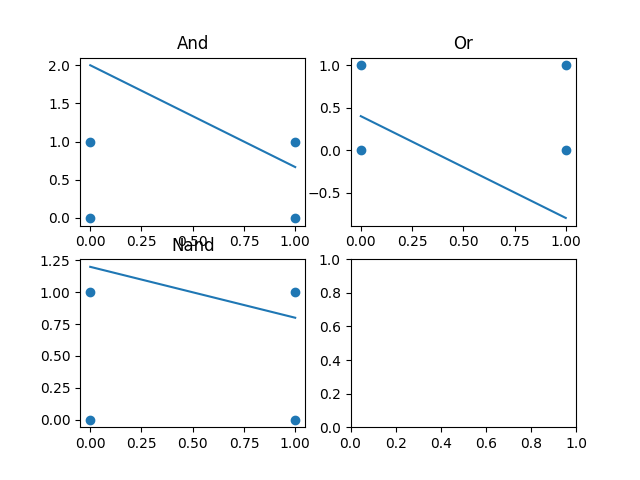
\includegraphics[scale = 1]{logic_gates.png}
  \caption{The results of the perceptron with logic gates}
\end{figure}

\newpage
\subsection{Classifying images}
Now lets try to do something more realistic we want to classify images with circles and rectangles
each image has a rectangle o a circle, we want to train the perceptron to be able to classifie each
of ones, so take a look these images, I know that the circles are not perfect but try to think that
they are circles.

\begin{figure}[H]
  \centering
  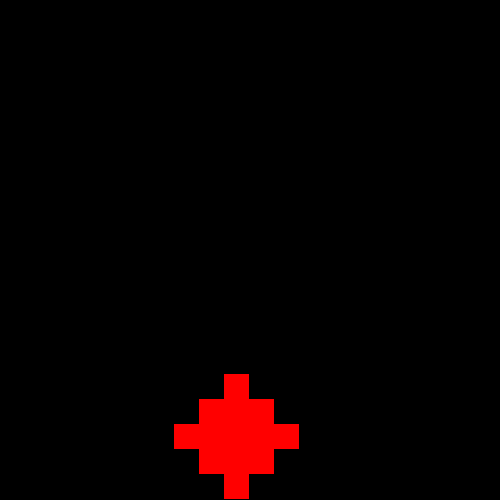
\includegraphics[scale = 0.4]{test_circle-2.png}
  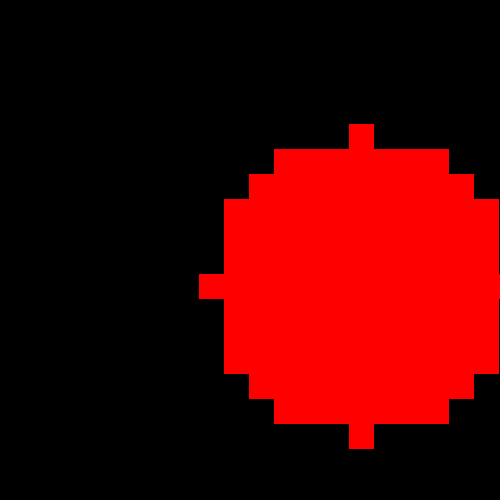
\includegraphics[scale = 0.4]{test_circle-23.png}
  \caption{Examples of circles}
\end{figure}

\begin{figure}[H]
  \centering
  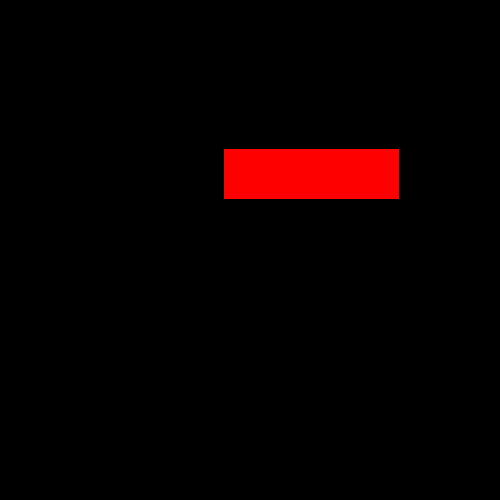
\includegraphics[scale = 0.4]{test_rect-39.png}
  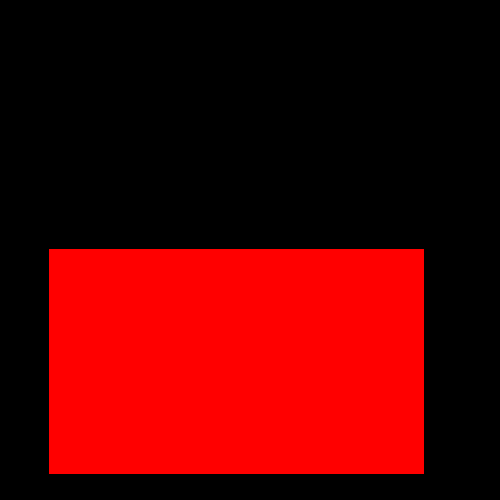
\includegraphics[scale = 0.4]{test_rect-13.png}
  \caption{Examples of rectangles}
\end{figure}
Each pixel represents an input, the images has a size of \textbf{20 x 20} pixels basically the perceptron
deals with \textbf{400} inputs then for each of these creates a weight, basically having
\textbf{400} weights, I know is too much, to train this kind of models is not easy because we
need to recollect massive datasets, for that reason I program this thing to have the capability to
generate its own dataset for its training, you can do that by manipulating the
\href{https://github.com/alecksandr26/machine-learning-code/blob/main/examples/perceptron_rectangle_circle/src/config.h}{config.h}.\\

The main idea of training and creating these kinds of models is to be used for problems where they
haven't been trained and be able to solve them, but obviously there is always going to be a
probability where the model gets a wrong answer, for that reason we always want to train this model
hardly with tons and tons of data.\\

You must  understand the larger our data set is, the less the probability of a wrong answer
from our model will be, and then after an hour of training the model, I tested with 1 hundred
random inputs where the neuron hadn't seen before and this was the result.
\begin{verbatim}
./main.out
 [INFO] Loading the brain
 [INFO] Brain detected
 [INFO] Brain loaded
 [INFO] Preparing the training data
 [INFO] Training data prepared
 [INFO] Training perceptron
 [INFO] Perceptron trained
 [INFO] Preparing the testing data
 [INFO] Testing data prepared
 [INFO] Testing perceptron
 [INFO] Perceptron tested
 [INFO] test fail data/test_rect-0.ppm
 [INFO] test fail data/test_rect-3.ppm
 [INFO] test fail data/test_circle-13.ppm
 [INFO] test fail data/test_rect-5.ppm
 [INFO] test fail data/test_circle-18.ppm
 [INFO] test fail data/test_rect-11.ppm
 [INFO] test fail data/test_rect-12.ppm
 [INFO] test fail data/test_circle-22.ppm
 [INFO] test fail data/test_circle-25.ppm
 [INFO] test fail data/test_circle-26.ppm
 [INFO] test fail data/test_rect-16.ppm
 [INFO] test fail data/test_rect-17.ppm
 [INFO] test fail data/test_rect-18.ppm
 [INFO] test fail data/test_rect-19.ppm
 [INFO] test fail data/test_rect-21.ppm
 [INFO] test fail data/test_circle-40.ppm
 [INFO] test fail data/test_rect-25.ppm
 [INFO] test fail data/test_rect-26.ppm
 [INFO] test fail data/test_rect-30.ppm
 [INFO] test fail data/test_circle-52.ppm
 [INFO] test fail data/test_circle-54.ppm
 [INFO] test fail data/test_rect-36.ppm
 [INFO] test fail data/test_rect-39.ppm
 [INFO] test fail data/test_rect-40.ppm
   76.0000000              76         100
 [INFO] Saving new brain
 [INFO] Brain saved
\end{verbatim}
And maybe the model needs more training or maybe it is because the problem is not linear separable,
we don't know, then I take all its \textbf{400} weights and put them in an image to have a graphical
representation of It's weights or It's brain.
\begin{figure}[H]
  \centering
  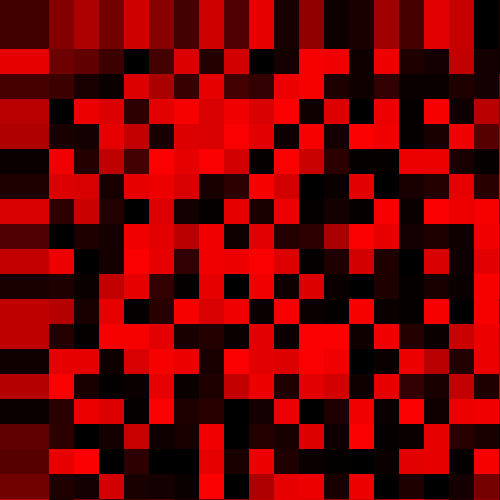
\includegraphics{brain.png}
  \caption{The brain of the perceptron.}
\end{figure}

\label{sec:problems-with-the-perceptron}
\section{The Problems with the Perceptron}
The main limitation of the perceptron, which sometimes renders it ineffective, is its inability to handle
non-linear problems. Identifying whether a problem is linear or not can be challenging since we can't easily
visualize hyperplanes in high-dimensional spaces. Consequently, no matter how extensively we train the
perceptron model, it will never converge for general cases.

However, by combining multiple perceptrons and organizing them into a larger structure, we can tackle these
non-linear problems. This arrangement compels each perceptron to focus on a specific pattern within the
broader problem, abstracting these patterns. It grants us the ability to classify non-linear problems,
effectively creating multiple hyperplanes for different aspects of the problem.

\begin{figure}[H]
  \centering
  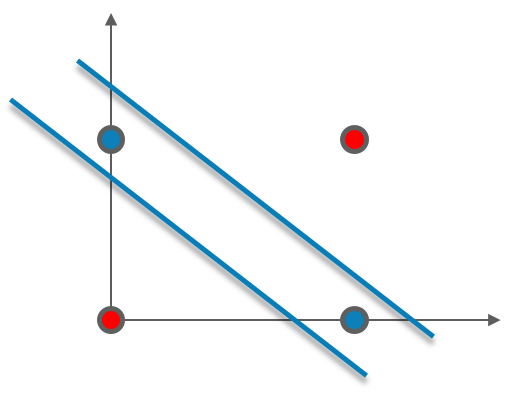
\includegraphics[scale = 0.5]{xor.png}
  \caption{A neural network dealing with XOR.}
\end{figure}

As illustrated above, we require three neurons to solve an XOR problem. One neuron learns the OR logic gate
pattern, another learns the NAND logic gate pattern, and both create hyperplanes to abstract the problem.
These abstractions are then fed into the third neuron, which only needs to apply the AND logic gate.

\begin{figure}[H]
  \centering
  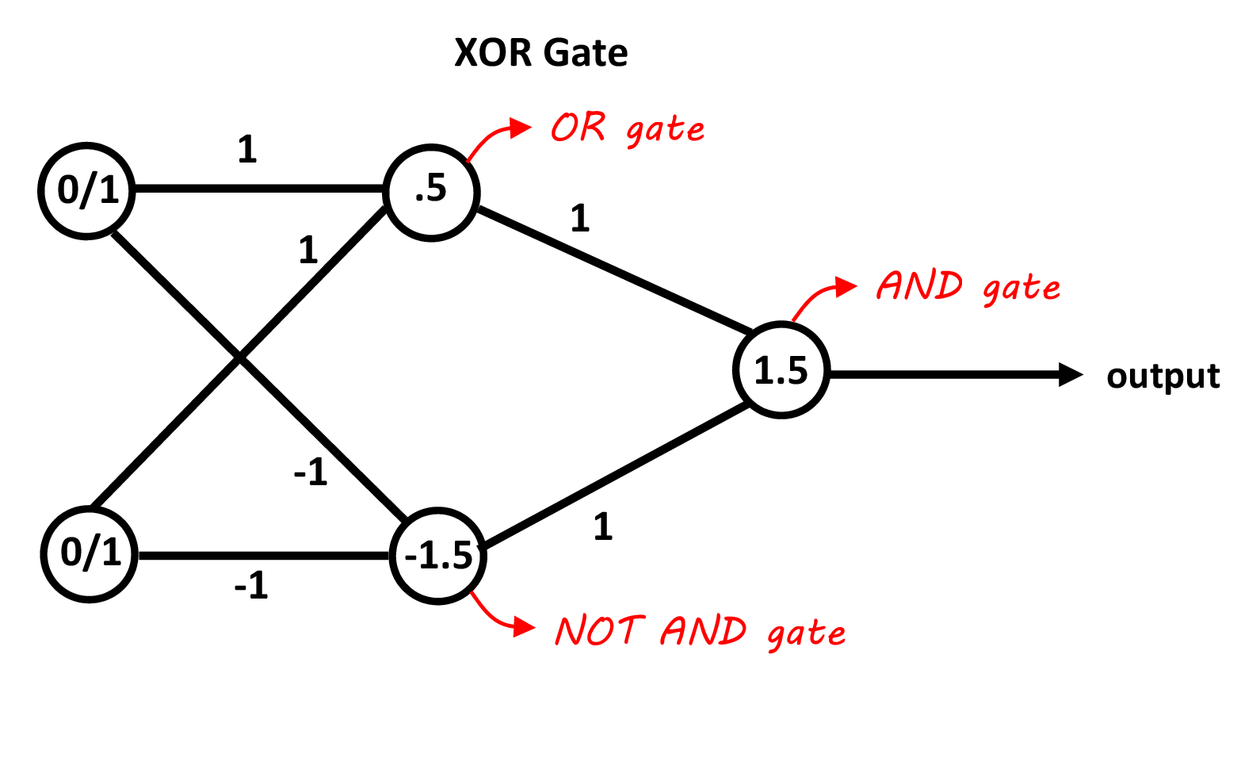
\includegraphics[scale = 0.5]{neurons.png}
  \caption{The structure of the neural network for XOR.}
\end{figure}

These structures are known as neural networks, and they become particularly interesting when we create
extensive arrangements of them.

Perceptrons are limited to linearly separable problems, meaning they can only learn to classify data that
can be separated by a hyperplane. However, they have served as building blocks for more complex neural
network architectures capable of handling intricate problems.

Overall, perceptrons are simple yet powerful tools for constructing basic binary classifiers. Their
contributions to the development of artificial intelligence and machine learning have been significant.



\Chapter{Predicting with an artificial neuron}{Introduction to linear regression}
\section{Classification and Prediction}
Artificial neurons can perform two different actions: classification and prediction. Originally, the idea of the
perceptron was to be a binary classifier, but it can actually do more. In this chapter, we will see how
to adapt the neuron to predict values, but first lets see what does exactly means classification and prediction.

\begin{itemize}
\item \textbf{Classification:} is the process of assigning a label to an input data point.
  For example, a classification model could be used to determine whether an email is spam or not spam, or
  whether a patient has a certain disease or not. We have already explored this concept in the previous chapter,
  where we provided examples using logic gates and a simple image classifier.
  
\item \textbf{Prediction:} is the process of estimating the value of a target variable based on a set of
  input variables. For example, a prediction model could be used to estimate the price of a house, or the
  likelihood of a customer clicking on an ad.
\end{itemize}

The perceptron can be utilized as a prediction model through a technique called linear regression.
Let's first delve into how linear regression works.

\subsection{How linear regression works?}
Linear regression is a statistical method that finds a linear relationship between the independent variables
and the dependent variable. This means that the relationship between the independent variables and
the dependent variable can be modeled by a straight line.\\
The independent variables are the variables that we believe influence the dependent variable. In the case
of predicting the price of a house, some independent variables might be the size of the house, the number of
bedrooms, the location of the house, and the age of the house.\\
The dependent variable is the variable that we are trying to predict. In the case of predicting the
price of a house, the dependent variable is the price of the house.\\
Linear regression can be geometrically represented as a line that best fits the data points in a dataset.
The independent variables are represented by the horizontal axis $\vec{x}$,
and the dependent variable is represented
by the vertical axis $y$. The line that best fits the data points is the one that minimizes the distance between
the line and the data points.


\begin{figure}[H]
  \centering
  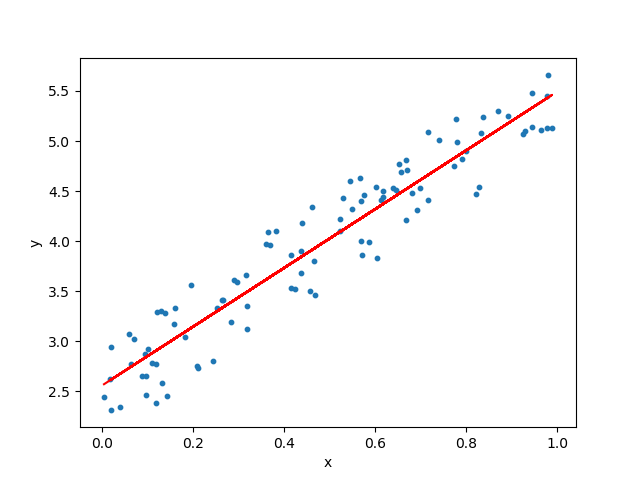
\includegraphics[scale = 0.38]{linear_regression.png}
  \caption{Linear regression.}
\end{figure}

The perceptron algorithm is a binary classifier that creates a linear decision boundary to separate data into two
categories. This is similar to linear regression, which also uses a linear boundary. However, linear regression
predicts continuous values, while the perceptron algorithm classifies data into distinct categories.
The perceptron learns from labeled examples to find the optimal boundary that separates the data effectively.

\begin{figure}[H]
  \centering
  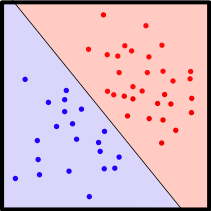
\includegraphics[scale = 0.8]{linearly.png}
  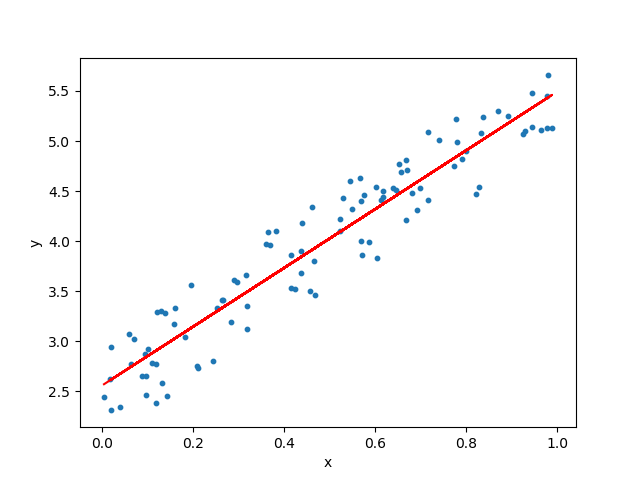
\includegraphics[scale = 0.4]{linear_regression.png}
  \caption{The linear separability and the linear regression}
\end{figure}

\section{Coding the prediction perceptron}
\subsection{Modifying the perceptron algorithm}
We have observed that the perceptron algorithm involves a dot product operation between the input components and
corresponding weights, given by $\sum_{i = 0}^n(x_i \cdot w_i) = \vec{x} \cdot \vec{w}$. Here,
$\vec{x} = \{1, x_1, x_2, \ldots, x_n\}$ represents the input vector, $\vec{w} = \{b, w_1, w_2, \ldots, w_n\}$
represents the weight vector, where $b = w_0$ and $1 = x_0$. This dot product is then passed through an
activation function.

We can express the output as $y = \text{activation}(\vec{x} \cdot \vec{w})$. The activation function maps the
result to a domain of $\{x_0, x_1\}$, depending on the chosen activation function.

To predict continuous values, we don't need an activation function because our outputs are not restricted to a
finite group of values like $\{x_0, x_1\}$. Instead, we require the entire domain, which can be represented
by $\mathbb{R}$ or $\mathbb{Z}$ depending on the type of value we are trying to predict. In some cases, we may
need to make convenient modifications to map values from $\mathbb{R}$ to another infinite group of values.

The algorithm can be simply understood as a dot product of vectors.
\[
f(\vec{x}) = \vec{w} \cdot \vec{x} \quad | \quad \vec{x} = \{1, x_1, \cdots, x_n\},
\vec{w} = \{b, w_1, \cdots, w_n \}
\]

\subsection{From linear regression algorithm to code}
First, declare your weights. Remember that the weights already include the bias or threshold, represented
as $\vec{w} = \{b, w_1, \cdots, w_n\}$. Therefore, you need to insert a value of 1 for each input data that you
want to provide to the perceptron, represented as $\vec{x} = \{1, x_1, \cdots, x_n\}$.
\begin{verbatim}
weights = [4.1, 0.0, 2.0, 1.0, 2.8] // 4.1 = b = w_0
input = [1.0, 23.0, 42.0, 12.0, 21.0] // 1.0 = x_0
\end{verbatim}
Next, you only need to sum and multiply each element and return the sum as it will represent the predicted value.
\begin{verbatim}
sum = 0.0
for (i = 0, i < input.length, i++)
    sum += input[i] * weights[i]
return sum
\end{verbatim}
The predicted value is computed through a dot product operation between the input vector and the weight vector.
This enables us to estimate continuous values and make predictions. To train this modified perceptron, we need
to adjust the weights. The training process involves iteratively updating the weights based on prediction
errors. 
\subsection{A simple training algorithm for predicting values}
To train a linear regression neuron, we can adjust the weights based on prediction errors.
In addition to the perceptron training algorithm, there are various approaches available for this purpose,
including popular ones like gradient descent and backpropagation, which will be covered extensively in the
subsequent chapters. These algorithms provide powerful techniques for refining the neuron's parameters and
optimizing its predictive performance. However, for our current focus on linear regression neurons, we will
utilize a modified version of the perceptron training algorithm. This modified approach allows us to
iteratively update the weights by considering the discrepancies $\varepsilon$ between predicted values and
the true target
values. By systematically adjusting the weights, we aim to minimize these prediction errors and improve the
accuracy of our linear regression neuron.
Actually, the learning algorithm we are going to use for this regression will be very similar to
the perceptron learning algorithm because
it shares almost the same characteristics. The main difference is that, for each iteration, it will update
the weights. Remember, our goal is to minimize the discrepancy, $\varepsilon$, as much as possible.
In simpler terms, the linear regression neuron learning process can be summarized in these three steps:
\begin{enumerate}
\item The training function makes predictions based on the activation function, which can be represented
  as $f(\vec{x}_t) = \vec{x}_t \cdot \vec{w}_k$, where $t$ denotes the current iteration through the training
  data, and $k$ represents the current state of the weights.

\item The perceptron for each $t$ iteration will adjusts its weights. Again there are different
  ways to perform this
  adjustment, but one common approach that we can use is to utilize useful information such as the input
  vector $\vec{x}$,
  the discrepancy, $\varepsilon$, which can be computed $\varepsilon = y_t - f(\vec{x}_t)$  where $y_t$ is the
  desired prediction,
  and a learning rate $\gamma$ (where $\gamma$ is a small value, $\gamma < 1$).
  The weight adjustment can be expressed as $\vec{w}_{k+1} = \vec{w}_k + \gamma \varepsilon \vec{x}_t$.

\item After many predictions and adjustments, the weights will converge to the desired weights denoted as
  $\vec{\theta}^*$, which can be represented as
  $k \rightarrow \infty \quad \implies \quad \vec{w}_k \rightarrow \vec{\theta}^*
  ,\quad \varepsilon \rightarrow 0$.
\end{enumerate}

By following these steps, the neuron learns and adapts its weights until it achieves accurate predictions.

\subsubsection{The Math Intuition of Linear Regression}
The goal of linear regression is to estimate the coefficients that best fit the observed data. In matrix notation
, the model can be represented as $y = X\beta + \varepsilon$, where $y$ is the vector of dependent variable
values,
$X$ is the matrix of independent variable values, $\beta$ is the vector of coefficients, and $\varepsilon$ is
the error term. The error term captures the discrepancy between the actual values of the dependent variable and
the values predicted by the linear regression model. By minimizing these discrepancies, the model aims to
find the
coefficients that provide the best overall fit to the data.
\begin{figure}[H]
  \centering
  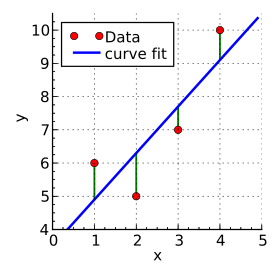
\includegraphics[scale = 1]{linear_regression2.png}
  \caption{In linear regression, the observations (red) are assumed to be the result of random deviations
    (green) from an underlying relationship (blue) between a dependent variable ($y$) and an independent
    variable ($x$).}
\end{figure}

\subsection{From Learning Algorithm to Code}
The learning algorithm we are going to use is similar to the perceptron learning algorithm.
First, you need to define the learning rate $\gamma$ and the number of iterations $t$ for training:
\begin{verbatim}
learning_rate = 0.01
num_epochs = 100
\end{verbatim}
The implementation of this training algorithm involves nested for loops, similar to the
perceptron learning algorithm. The `inputs` array should be a bidimensional array.

\begin{verbatim}
for (i = 0; i < num_epochs; i++)
    for (j = 0; j < inputs.length; j++)
        sum = 0.0;
        for (k = 0; k < weights.length; k++)
            sum += inputs[j][k] * weights[i];
\end{verbatim}
Within the innermost loop iterating over the inputs, you will update the weights:
\begin{verbatim}
error = output[j] - sum;
for (k = 0; k < weights.length; k++)
    weights[k] += learning_rate * error * inputs[j][k];
\end{verbatim}
This code segment outlines the general structure of the learning algorithm.

\section{The math behind of the learning algorithm}
When using the linear regression neuron for prediction instead of classification, there will always
be a discrepancy, denoted as $\varepsilon$. This discrepancy can be calculated as follows:
\[
\varepsilon_t = y_t - \vec{w}_k \cdot \vec{x}_t
\]
Ultimately, our goal is to find a desired vector $\vec{\theta}^*$ that minimizes the
discrepancy $\varepsilon$ for all possible inputs. Mathematically, this can be expressed as:
\[
\exists \vec{\theta}^* \in \mathbb{R}^{d} \quad|\quad \forall \text{min}\{\varepsilon_t\}
\]
where
\[
\varepsilon_t = y_t - \vec{\theta}^* \cdot \vec{x}_t\quad|\quad \forall(\vec{x}_t, y_t) \in \mathbb{D}
\]
Here, $(\vec{x}_t, y_t) \in \mathbb{D}$ represents the entire dataset.

The fundamental idea is to utilize $\varepsilon_t$ as a direction and proportion to iteratively
adjust the weights, resulting in an update equation like this:
\[
\vec{w}_{k + 1} = \vec{w}_{k} + \varepsilon_t \cdot \vec{x}_t
\]
Intuitively, consider the following expressions:
\[
\varepsilon_t < 0 \Longleftrightarrow y_t < \vec{w}_k \cdot \vec{x}_t
\Longleftrightarrow \vec{w}_{k + 1} < \vec{w}_k
\]

\[
\varepsilon_t > 0 \Longleftrightarrow y_t > \vec{w}_k \cdot \vec{x}_t
\Longleftrightarrow \vec{w}_{k + 1} > \vec{w}_k
\]

In the algorithm, we aim to make the weight adjustments less aggressive.
To understand why we adjust the weights in this manner, consider the following illustration.

\begin{center}
\begin{tikzpicture}[scale=1.5]
  \draw[thick,->] (2,0) -- (0,1) node[anchor=south west]{$\vec{w}_k$};
  \draw[thick,->] (2,0) -- (5,0) node[anchor=south west]{$\vec{\theta}^*$};
\end{tikzpicture}
\end{center}

Here, $\vec{\theta}^*$ represents the desired vector configuration, while $\vec{w}_k$ corresponds to the
current iteration's weights. Although we do not know the exact position of $\vec{\theta}^*$, we
can approximate $\vec{w}_k$ to $\vec{\theta}^*$ by adding vectors. Consequently, we can introduce
the vector $\varepsilon_t \cdot \vec{x}_t$ to the illustration.

\begin{center}
\begin{tikzpicture}[scale=1.5]
  \draw[thick,->] (2,0) -- (0,1) node[anchor=south west]{$\vec{w}_k$};
  \draw[thick,->] (2,0) -- (5,0) node[anchor=south west]{$\vec{\theta}^*$};
  \draw[thick,->] (2,0) -- (5,-1) node[anchor=south west]{$\varepsilon_t\vec{x}_t$};
\end{tikzpicture}

\begin{tikzpicture}[scale=1.5]
  \draw[thick,->] (2,0) -- (0,1) node[anchor=south west]{$\vec{w}_k$};
  \draw[thick,->] (2,0) -- (5,0) node[anchor=south west]{$\vec{\theta}^*$};
  \draw[thick,->] (2,0) -- (5,-1) node[anchor=south west]{$\varepsilon_t\vec{x}_t$};

  \draw let \p1 = (-2,1), \p2 = (5,-1.78), \n1 = {atan2(\y1,\x1)}, \n2 = {atan2(\y2,\x2)} in (2,0) + (\n1:0.8) arc (\n1:\n2:0.8) node[midway, above right] {$\theta$};
\end{tikzpicture}
\end{center}

Recall that adding two vectors together results in their rotation. Hence,
the computation of $\vec{w}_{k + 1}$ must bring it closer to $\vec{\theta}^*$.


So think in the addition of vector as way to rotate a vector, look if I sum $\vec{w}_k + \varepsilon_t\vec{x}_t$
I get the next iteration the $k + 1$ iteration which results on this new vector $\vec{w}_{k + 1}$.
\begin{center}
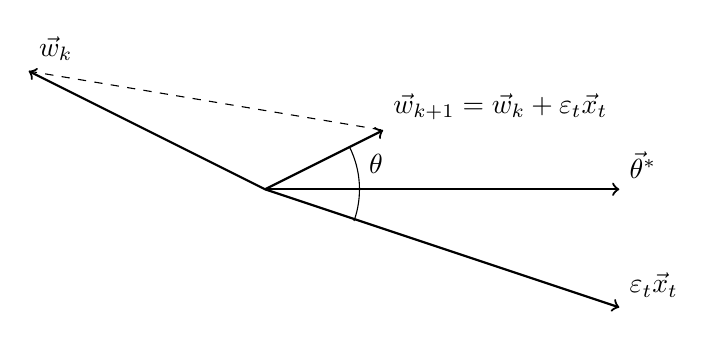
\begin{tikzpicture}[scale=1.5]
  \draw[thick,->] (2,0) -- (0,1) node[anchor=south west]{$\vec{w}_k$};
  \draw[thick,->] (2,0) -- (5,0) node[anchor=south west]{$\vec{\theta}^*$};
  \draw[thick,->] (2,0) -- (5,-1) node[anchor=south west]{$\varepsilon_t\vec{x}_t$};
  \draw[thick,->] (2,0) -- (3,0.5) node[anchor=south west]{$\vec{w}_{k + 1} = \vec{w}_k + \varepsilon_t\vec{x}_t$};
  \draw[dashed] (0,1) -- (3,0.5);
  
  \draw let \p1 = (2,1), \p2 = (5,-1.78), \n1 = {atan2(\y1,\x1)}, \n2 = {atan2(\y2,\x2)} in (2,0) + (\n1:0.8) arc (\n1:\n2:0.8) node[midway, above right] {$\theta$};
\end{tikzpicture}
\end{center}

Finally, through the \hyperref[sec:perceptron-convergence-proof]{convergence proof of the perceptron},
we can be confident that
$\vec{w}_k$ will converge to the desired vector of weights, $\vec{\theta}^*$.

\section{Examples}
By comprehending the underlying linear regression algorithm
and its convergence properties, we have uncovered the key principles
behind its functionality. The availability of practical code examples further enhances our understanding and
allows for easy implementation. You can find a collection of these illustrative examples in the provided
GitHub repository at the following link:
\href{https://github.com/alecksandr26/fortran-ml/tree/main/examples}{examples}.
\subsection{Linear regression neuron module in fortran}
I have developed a simple linear regression neuron  module in Fortran, which includes the weights.
The module encompasses subroutines for training and testing the
neuron. To delve deeper into the implementation details, you can access the source code
\href{https://github.com/alecksandr26/fortran-ml/tree/main/src/mod_linear_regression.f90}{here}.

\begin{lstlisting}
module mod_linear_regression
  use iso_fortran_env, only : real32, int32
  use assertf
  implicit none

  private
  public lr_init, lr_free, linear_regression, lr_train, lr_test

  type linear_regression
     integer(int32) :: n
     real(real32), pointer :: w(:)
  end type linear_regression
  
contains
  
  subroutine lr_init(lr, w)
    real(real32), intent(in) :: w(:)
    type(linear_regression), intent(out) :: lr

    ! Fetch the size from the array
    lr%n = size(w)

    allocate(lr%w(lr%n))
    
    ! Copy the initial weights 
    lr%w(:) = w(:)
  end subroutine lr_init

  subroutine lr_free(lr)
    type(linear_regression), intent(in out) :: lr
    deallocate(lr%w)
    lr%n = 0
  end subroutine lr_free

  subroutine lr_train(lr, inputs, outputs, lrate, nepochs)
    type(linear_regression), intent(in out) :: lr
    real(real32), intent(in) :: inputs(:, :), outputs(:)
    real(real32), intent(in) :: lrate
    integer(int32), intent(in) :: nepochs

    integer(int32) :: n
    real(real32), allocatable :: results(:)
    integer(int32) :: i, j, k
    
    n = size(outputs)
    allocate(results(n))

    do concurrent(i = 1 : nepochs)
       do concurrent(j = 1 : n)
          ! Vector multiplication w * x
          results(j) = 0
          do concurrent(k = 1 : lr%n)
             results(j) = results(j) + lr%w(k) * inputs(k, j)
          end do

          ! Update the weights
          do concurrent(k = 1 : lr%n)
             lr%w(k) = lr%w(k) + lrate * (outputs(j) - results(j)) * inputs(k, j)
          end do
       end do
    end do
    deallocate(results)
  end subroutine lr_train

  subroutine lr_test(lr, input, output)
    type(linear_regression), intent(in out) :: lr
    real(real32), intent(in) :: input(:)
    real(real32), intent(out) :: output
    integer(int32) k

    do concurrent(k = 1 : lr%n)
       output = output + lr%w(k) * input(k)
    end do
  end subroutine lr_test
  
end module mod_linear_regression
\end{lstlisting}

\subsection{Predicting sales}
This scenario involves a fundamental prediction task: estimating the potential earnings of a product or
service after a specific number of days of sales, such as forecasting the revenue generated after 11 days.
In such cases, linear regression emerges as the ideal approach for making accurate predictions. With its
ability to capture linear relationships between variables, linear regression proves to be a suitable candidate
for predicting future outcomes in this context.\\

In this simple program written in Fortran, I utilized the previously demonstrated Fortran module for performing
linear regression. In basic terms, the program prints the data being used and proceeds to predict the output
for each input, displaying the results.
\begin{lstlisting}
program example
  use iso_fortran_env, only : real32, int32
  use mod_linear_regression
  use assertf
  implicit none

  type(linear_regression) :: lr
  real(real32) :: inputs(2, 7) = reshape([1, 4, 1, 5, 1, 6, 1, 7, 1, 8, 1, 9, 1, 10], [2, 7])
  ! inputs = [[1, 4], [1, 5], [1, 6], [1, 7], [1, 8], [1, 9], [1, 10]]
  real(real32) :: outputs(7) = [50, 70, 72, 73, 90, 95, 105]
  real(real32) :: output = 0.0
  integer(int32) :: i = 0

  write(*, '(A)', advance='no') "inputs: "
  do i = 1, size(inputs, 2)
     write(*, '(F0.1, A)', advance='no') inputs(2, i), ' '
  end do
  write(*,*)

  write(*, '(A)', advance='no') "outputs: "
  do i = 1, size(outputs)
     write(*, '(F0.1, A)', advance='no') outputs(i), ' '
  end do
  write(*,*)
  

  call lr_init(lr, [0.0, 0.0])
  call lr_train(lr, inputs, outputs, 0.0001, 4000000)

  write(*, '(A)', advance='no') "results: "
  do i = 1, size(inputs, 2)
     call lr_test(lr, inputs(:, i), output)
     write(*, '(F0.1, A)', advance='no') output, ' '
     output = 0.0
  end do
  write(*,*)

  write(*, '(A)', advance='no') "weights: "
  write(*, '(F0.1, A, F0.1)', advance='no') lr%w(1), ' ', lr%w(2)
  write(*,*)
  
  call lr_free(lr)
end program example 
\end{lstlisting}
The module of linear regression works as the \hyperref[sec:perceptron-module-fortran]{perceptron module}.

\subsubsection{Output}
\begin{verbatim}
inputs: 4.0 5.0 6.0 7.0 8.0 9.0 10.0 
outputs: 50.0 70.0 72.0 73.0 90.0 95.0 105.0 
results: 54.3 62.6 70.9 79.3 87.6 95.9 104.3 
weights: 21.0 8.3  
\end{verbatim}
\subsubsection{Picture of the results}
This is the result of the line. As you can see, the neuron learns after iterating with a lot of epochs.

\begin{figure}[H]
  \centering
  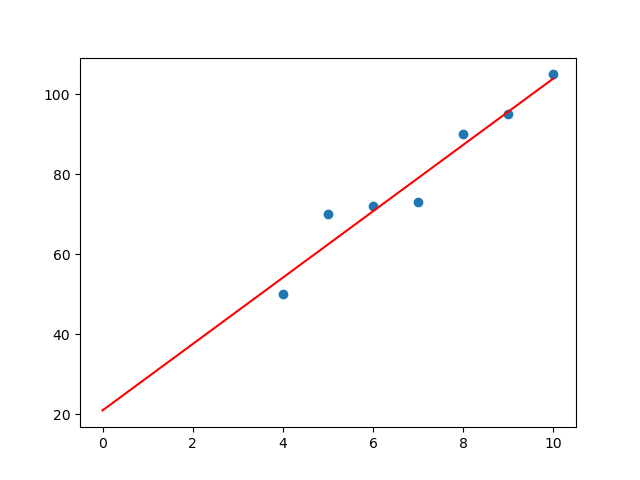
\includegraphics[scale = 0.9]{sales_prediction.png}
  \caption{Results of the linear regression neuron.}
\end{figure}

\subsection{Stock price prediction}
In the previous chapter, we delved into a simple example to grasp the fundamentals. Now, let's take on a more
realistic scenario. To accomplish this, we'll work with the 'TESLA.csv' file, which can be accessed through the
provided link. This file contains a comprehensive dataset encompassing various aspects of Tesla's stock prices,
including significant labels such as Date, Open, High, Low, Close, Adj Close, and Volume.

Our objective is to predict the closing price of Tesla's stock by considering multiple factors. These factors
include the date, represented as a numerical value, along with the opening price, high price, low price, and
volume of stocks exchanged.

Let's take a closer look at the initial lines of the .csv file:
\begin{verbatim}
Date,Open,High,Low,Close,Adj Close,Volume
2020-01-02,84.900002,86.139999,84.342003,86.052002,86.052002,47660500
2020-01-03,88.099998,90.800003,87.384003,88.601997,88.601997,88892500
2020-01-06,88.094002,90.311996,88.000000,90.307999,90.307999,50665000
2020-01-07,92.279999,94.325996,90.671997,93.811996,93.811996,89410500
2020-01-08,94.739998,99.697998,93.646004,98.428001,98.428001,155721500
2020-01-09,99.419998,99.760002,94.573997,96.267998,96.267998,142202000
2020-01-10,96.358002,96.987999,94.739998,95.629997,95.629997,64797500
2020-01-13,98.699997,105.125999,98.400002,104.972000,104.972000,132588000
2020-01-14,108.851997,109.482002,104.980003,107.584000,107.584000,144981000
\end{verbatim}
Training this type of neuron posed challenges due to the complexity of achieving linear separability.
The initial hurdle I encountered was determining the appropriate learning rate. Since these models learn by
iteratively adjusting weights based on nearly random differences, selecting an unsuitable learning rate could
prevent convergence. Consequently, a second issue arose: striking a balance between convergence and training
time. To ensure convergence, I had to opt for an extremely small learning rate, which in turn necessitated a
substantial number of epochs. As a result, I spent countless hours training the model without achieving
satisfactory outcomes. To illustrate, consider the accompanying images: the red dots represent predicted
values, while the blue dots represent actual values.

\begin{figure}[H]
  \centering
  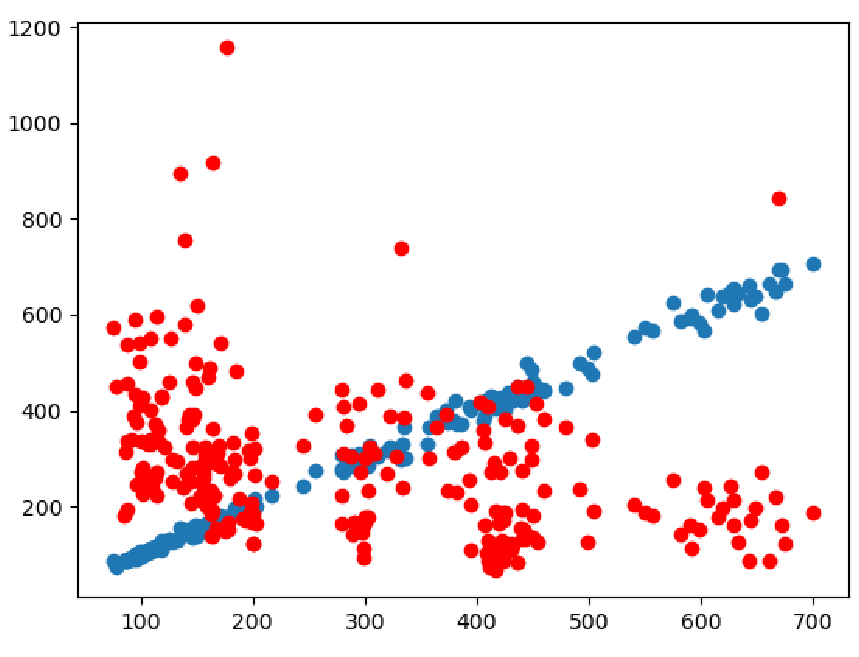
\includegraphics[scale = 0.4]{stock_prediction2.png}
  \caption{Results of the linear regression neuron predicting the stock.}
\end{figure}

As you can observe from the results, the predictions obtained were not satisfactory. In an attempt to improve
the model's performance, a decision was made to remove one of the independent variables, namely the Volume.
This reduction resulted in a model with four dimensions, including a bias term. Consequently, the task at
hand involved training and fitting five weights.\\

After investing a considerable amount of time in training the model, notable progress was achieved. The
predictions exhibited significant improvement, accurately capturing the underlying patterns and relationships
within the variables. This successful outcome underscores the effectiveness of the model and its ability to
make robust predictions.

\begin{figure}[H]
  \centering
  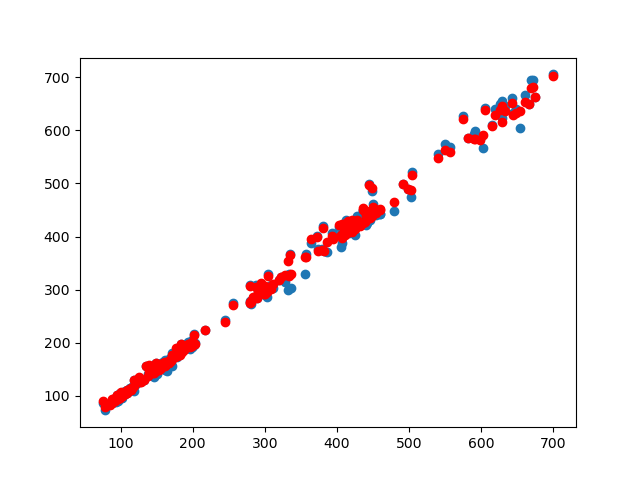
\includegraphics[scale = 0.9]{stock_prediction.png}
  \caption{Results of the linear regression neuron predicting the stock.}
\end{figure}

Something additional that could enhance the realism of our predictions is incorporating the concept of
prediction intervals. By considering the minimum and maximum discrepancies observed during training, we can
construct a range, denoted as $[min(\varepsilon_t), max(\varepsilon_t)]$, where $\varepsilon_t$ represents the
prediction error for a given observation. After making a prediction, we can introduce a random noise component
drawn from this range to add variability and make the predictions more realistic. It is crucial to pay
attention to this aspect if we aim to generate accurate and reliable predictions.

\section{The problems with a linear regression neuron}
 training prediction neurons poses a greater challenge compared
to classification neurons. The task of prediction involves an infinite approximation, striving to create a
model that can predict outcomes with minimal error, ideally achieving $\varepsilon = 0$. However, in
real-world
scenarios, perfect predictions are seldom attainable due to the inherent complexity and non-linearity of the
underlying problems. As we explored in the previous chapter, real-world data rarely exhibits a perfectly
straight pattern, making it more difficult to develop accurate prediction models. Consequently, we often
encounter the need to incorporate additional neurons and employ advanced techniques to effectively handle
these non-linear problems and achieve more realistic predictions. While delving into the depths of non-linear
problems is beyond the scope of this discussion, it is worth noting that the solution lies in utilizing more
neurons and constructing more complex structures to minimize the error term $\varepsilon \approx 0$. To echo the
sentiments expressed in the previous chapter, the necessity for more neurons and sophisticated architectures
becomes apparent. Thus, I won't delve deeper into this topic since it was thoroughly addressed
\hyperref[sec:problems-with-the-perceptron]{in the
previous chapter}.


\Chapter{Gradient Descent}{Optimizing learning algorithms}



\section{What is it?}
\subsection{A little bit of history}
Before delving into the gradient descent algorithm, I recommend studying a bit of calculus,
specifically differential calculus. Now, let's take a moment to explore the history of the perceptron.\\

The perceptron, invented in 1943 by Warren McCulloch and Walter Pitts, is a fundamental concept in
artificial neural networks. In 1958, Frank Rosenblatt built the first implementation known as the "Mark 1
perceptron" at the Cornell Aeronautical Laboratory. It was initially designed as a machine for image recognition,
featuring an array of 400 photocells connected to neurons with weight updates performed by electric motors.\\

Rosenblatt's bold claims about the perceptron during a 1958 press conference sparked controversy.
The New York Times reported his statement that the perceptron was the "embryo of an electronic computer"
capable of various human-like abilities. This fueled speculation about the potential of perceptron-based
systems.\\

However, it is important to acknowledge the limitations of the perceptron. One such limitation is the
potentially slow training process, often requiring a significant number of iterations to achieve convergence.
Furthermore, the perceptron may struggle to provide accurate predictions, especially when faced with complex and
nonlinear problems. As I have demonstrated through various examples, these limitations highlight the need for
alternative neural network architectures and advanced learning algorithms to overcome these challenges and
improve prediction accuracy. It is crucial to consider these factors when applying the perceptron or exploring
other approaches in the field of artificial intelligence.

\subsection{First approach to the algorithm}
\subsubsection{How we can measure the error from our models?}
Before delving into the gradient descent algorithm, let's address the question of how to measure this error.
In our previous discussions, we derived an expression that enables us to evaluate and update the weights of
our model. This expression serves as a means to assess the discrepancy between the predicted outputs of our
model and the actual outcomes. By utilizing this error measurement, we optimize the weights
to improve the accuracy of our model.
\[
\varepsilon_t = y_t - (\vec{x}_t \cdot \vec{w}_k)
\]
However, this measurement only works for a single input and output, which is not quite useful if we want to
understand the overall accuracy of our model across the entire dataset. To address this limitation, the
first approach that comes to mind is to sum all the potential $\varepsilon_t$ values from our dataset.
\[
\sum_{t = 1}^{n}(y_t - (\vec{x}_t \cdot \vec{w}_k))
\]
The challenge with this calculation is that the resulting values can have both positive and negative signs,
which makes interpretation challenging. To address this issue, we can take the absolute value of each
$\varepsilon_t$, considering only the magnitude of the error. Additionally, we can normalize the error
by scaling it with
$\frac{1}{n}$, where $n$ represents the number of data inputs. This normalization ensures a consistent and
meaningful measure of the error.
\[
\frac{1}{n} \cdot \sum_{t = 1}^{n}|(y_t - (\vec{x}_t \cdot \vec{w}_k))|
\]
Now, this expression proves to be highly valuable in measuring the error of our model. It further emphasizes
the significance of utilizing a substantial amount of data. By incorporating a large and diverse dataset, we
can obtain more comprehensive and reliable error measurements, enhancing our understanding of the model's
performance.\\

This expression is the key to optimizing our learning algorithm for both types of neurons. As this expression
approaches zero, it indicates that we are getting closer to finding the most optimal weights. It serves as a
critical indicator of our model's performance and guides us in refining our learning process.
\[
\frac{1}{n} \cdot \sum_{t = 1}^{n}|(y_t - (\vec{x}_t \cdot \vec{w}_k))|\quad \rightarrow \quad 0
\quad \implies \quad \vec{w}_k \quad \rightarrow \quad \vec{\theta}^*
\]
It is important to remember that $\vec{\theta}^*$ represents the desired optimal weights. This expression is
commonly referred to as the \textbf{Mean Absolute Error}, which quantifies the average magnitude of the errors
in our model's predictions.
\subsubsection{How we can use this expression?}
Before diving into the details, I recommend taking some time to study calculus concepts such as derivatives, as
they
will be essential in understanding the algorithm. Now, let's proceed. We can envision the Mean Absolute Error
as a function of the weight vector $\vec{w}_k$.
\[
MAE(\vec{w}) = \frac{1}{n} \cdot \sum_{t = 1}^{n}|(y_t - (\vec{x}_t \cdot \vec{w}))|
\]
Then let me ask you a question: What is the graph representation of an absolute value function? Well, this is it.
\begin{center}
\begin{tikzpicture}[scale=1.5]
  % Axis
  \draw[->] (-2,0) -- (2,0) node[right] {$\vec{w}$};
  \draw[->] (0,-2) -- (0,2) node[above] {$MAE$};

  % Absolute value function
  \draw[domain=-2:2,smooth,variable=\x,blue] plot ({\x},{abs(\x)});
\end{tikzpicture}
\end{center}

We know that we start with random weights, and those are our initial weights $\vec{w}_0$. We can plot this
vector on our graph, which may look like this. However, it is important to note that this graph is based on
the assumption that all values of $\vec{w}$ lie along a single line.

\begin{center}
\begin{tikzpicture}[scale=1.5]
  % Axis
  \draw[->] (-2,0) -- (2,0) node[right] {$\vec{w}$};
  \draw[->] (0,-2) -- (0,2) node[above] {$MAE$};

  % Absolute value function
  \draw[domain=-2:2,smooth,variable=\x,blue] plot ({\x},{abs(\x)});

  % w0
  \draw[dashed] (-1,0) node[below] {$\vec{w}_0$} -- (-1,1);
  
  % Dot for w0
  \filldraw[red] (-1,1) circle (1pt);

  % Output of MAE(w0)
  \draw[dashed] (0,1)  -- (-1, 1) node[left] {$MAE(\vec{w}_0)$};
\end{tikzpicture}
\end{center}
From this perspective of the graph, we can clearly identify the location of the optimal weights $\vec{\theta}^*$.
\begin{center}
\begin{tikzpicture}[scale=1.5]
  % Axis
  \draw[->] (-2,0) -- (2,0) node[right] {$\vec{w}$};
  \draw[->] (0,-2) -- (0,2) node[above] {$MAE$};

  % Absolute value function
  \draw[domain=-2:2,smooth,variable=\x,blue] plot ({\x},{abs(\x)});

  % w0
  \draw[dashed] (-1,0) node[below] {$\vec{w}_0$} -- (-1,1);
  
  % Dot for w0
  \filldraw[red] (-1,1) circle (1pt);

  % Output of MAE(w0)
  \draw[dashed] (0,1)  -- (-1, 1) node[left] {$MAE(\vec{w}_0)$};
  
  \filldraw[red] (0, 0) circle (2pt) node[below right] {$\vec{\theta}^*$};
\end{tikzpicture}
\end{center}

Our final question is whether there is a way to determine the path from any random
$\vec{w}_0$ to $\vec{\theta}^*$, as it appears to be possible from this perspective. We need to identify
the direction and trajectory to reach the optimal weights.

\begin{center}
\begin{tikzpicture}[scale=1.5]
  % Axis
  \draw[->] (-2,0) -- (2,0) node[right] {$\vec{w}$};
  \draw[->] (0,-2) -- (0,2) node[above] {$MAE$};

  % Absolute value function
  \draw[domain=-2:2,smooth,variable=\x,blue] plot ({\x},{abs(\x)});

  % w0
  \draw[dashed] (-1,0) node[below] {$\vec{w}_0$} -- (-1,1);
  
  % Dot for w0
  \filldraw[red] (-1,1) circle (1pt);

  % Output of MAE(w0)
  \draw[dashed] (0,1)  -- (-1, 1) node[left] {$MAE(\vec{w}_0)$};
  
  \filldraw[red] (0, 0) circle (2pt) node[below right] {$\vec{\theta}^*$};

  % Arrow from w0 to Theta*
  \draw[->, red] (-1, -0.4) -- (-0.1, -0.4);
\end{tikzpicture}
\end{center}
The answer to that question is the gradient descent algorithm. Gradient descent is an optimization algorithm
that, given a function, not only finds a direction towards its local minimum value but also determines a better
proportion for the updates. In our example, the local minimum value corresponds to $\vec{\theta}^*$. By following
the direction and proportion
indicated by the gradient descent algorithm, we update our weights, consistently moving towards the
local minimum position. This is the fundamental concept behind the algorithm.

\section{Diving into the algorithm}
\label{sec:diving_into_the_algorithm}
direction and magnitude of weight adjustments? This was the final question we addressed in the previous
section. The solution lies within the gradient descent algorithm, but how does it solve it? It is solved by
utilizing the realm of calculus. Through calculus, we can optimize our approach by identifying the minimum
and maximum points of a function. If you have completed the homework assigned at the beginning of this
chapter, you will grasp the concept that the derivative of a function at a specific point represents the
rate of change of that function, which makes sense because the notation of derivatives, introduced by
Gottfried Wilhelm Leibniz, represents a fraction or a rate.
\[
\frac{d}{dx}(f(x)) = \lim_{h \rightarrow 0}\frac{f(x + h) - f(x)}{h}
\]
Then, I have been withholding something that you might have already noticed if you studied as I suggested
earlier. The absolute function, $f(x) = |x|$, is not a differentiable function, which poses a challenge when
using calculus in our approach. To leverage calculus effectively, we require differentiable functions that
exhibit continuity. The absolute value function lacks continuity at $x \rightarrow 0$, so it is not
usefull.\\

Fortunately, there is an alternative approach. By replacing the absolute value function with a second-degree
polynomial, we can achieve a similar effect. This modified expression is known as the Mean Square Error. With
the Mean Square Error, we address the issue of continuity and arrive at our algorithm.
\[
MSE(\vec{w}) = \frac{1}{n} \cdot \sum_{t = 1}^{n}(y_t - (\vec{x}_t \cdot \vec{w}))^2
\]
The graph of this function would resemble something like this, considering the perspective of $\vec{w}$
as a single variable.
\begin{center}
\begin{tikzpicture}[scale=1.5]
  % Axis
  \draw[->] (-2,0) -- (2,0) node[right] {$\vec{w}$};
  \draw[->] (0,-2) -- (0,4) node[above] {$MSE$};

  % Square function
  \draw[domain=-2:2,smooth,variable=\x,blue] plot ({\x},{\x*\x});

  % w0
  \draw[dashed] (-1,0) node[below] {$\vec{w}_0$} -- (-1,1);
  
  % Dot for w0
  \filldraw[red] (-1,1) circle (1pt);

  % Output of MSE(w0)
  \draw[dashed] (0,1)  -- (-1, 1) node[left] {$MSE(\vec{w}_0)$};
  
  \filldraw[red] (0, 0) circle (2pt) node[below right] {$\vec{\theta}^*$};
\end{tikzpicture}
\end{center}

This approach is immensely valuable as it provides us with information regarding the direction in which to
move and the appropriate magnitude of weight updates. Consider this logical reasoning: the derivative guides
us towards optimal weight adjustments, enabling us to make informed decisions about how much to modify the
weights. Let's follow the next example: We want to iteratively find the minimum value of that function.

\[
f(x) = x^2,\quad x_0 = 5
\]

\[
\frac{d(f(x))}{dx}(x_0) = 2 \cdot x_0 = 10 > 0
\]
Here I define my learning reate $\gamma$.
\[
\gamma = 0.1
\]
Notice that I'm subtracting the value of the derivative multiplied by the learning rate $\gamma$.
\[
x_1 = x_0 - \gamma * \frac{d(f(x))}{dx}(x_0) = 5 - 0.1 = 4.9
\]
Then, if we repeat this process until $n = 100$, we will obtain results like these.
\[
x_{100} = 1.0185179881672439\cdot10^{-9} = 0.0000000010185179881672439
\]
Generally, that is the basic idea behind the gradient descent algorithm. However, it's not as straightforward
as it seems. Since our function takes a vector $\vec{w}$ as an input, traditional derivatives for abstract
vectors do not exist. Instead, we utilize partial derivatives, denoted as $\frac{\partial f}{\partial x_1}$,
to approximate the concept. Another important concept is the gradient, represented by the nabla symbol
($\nabla$), which encompasses the partial derivatives in vector form.
\[
\nabla MSE(\vec{w}) =
\begin{bmatrix} \frac{\partial MSE}{\partial w_1}(\vec{w})
  \\ \vdots
  \\ \frac{\partial MSE}{\partial w_m}(\vec{w})
\end{bmatrix}
\]
This is where things start to get more complex. I recommend studying calculus, specifically the chain rule,
as we will be using it. When all components of the gradient approach zero,
$\nabla MSE(\vec{w}) = [0, \cdots, 0]$, we have found our desired vector of weights, $\vec{\theta}^*$.
Graphically, it may look like this.

\begin{center}
\begin{tikzpicture}
\begin{axis}[
  xlabel=$\vec{w}$,
  ylabel=$MSE(\vec{w})$,
  xmin=-5,xmax=5,
  ymin=-1,ymax=10,
  axis lines=center,
  domain=-3:3,
  samples=100,
  xtick=\empty, % removes numbers from x-axis
  ytick=\empty, % removes numbers from y-axis
]
\addplot+[mark=none] {x^2+2};
\node[label={below left:$\vec{\theta}^*$}, circle, fill, inner sep = 2pt, red] at (axis cs:0,0) {};
\draw[thick] (250, 30) -- (750, 30);
\node[label={below left:$\scriptstyle \nabla MSE(\vec{\theta}^*) = [0, \cdots, 0]$}] at (axis cs:0,2) {};
\end{axis}
\end{tikzpicture}
\end{center}

Utilizing each of these partial differences as finite differences enables us to cover all the components of
the gradient descent algorithm. However, let's delve deeper into these concepts and explore the gradient
descent method more thoroughly. To begin, let's revisit the meaning of $\vec{x}_t \cdot \vec{w}$, which
represents the dot product between $\vec{x}_t$ and $\vec{w}$.
\[
\vec{x}_t \cdot \vec{w} = \sum_{i = 1}^{m} x_{t, i} \cdot w_i = (x_{t, 1} \cdot w_1 + \cdots + x_{t, m} \cdot w_m)
\]
Where $m$ is the number of components that each vector has, so if we replace this into our definition
$MSE(\vec{w})$ we could arrive to this expression.
\[
MSE(\vec{w}) = \frac{1}{n} \cdot \sum_{t = 1}^{n}(y_t - \sum_{i = 1}^{m}x_{t, i} \cdot w_i)^2
= \frac{1}{n} \cdot ((y_1 - \sum_{i = 1}^{m}x_{1, i} \cdot w_i)^2 + \cdots + (y_n - \sum_{i = 1}^{m}x_{n, i} \cdot w_i)^2)
\]
To avoid the need for finite differences and arrive at a more concise expression, we can leverage the
chain rule. For instance, we can define.
\[
u_t = y_t - \vec{x}_t \cdot \vec{w} = y_t - \sum_{i = 1}^{m}x_{t, i} \cdot w_i
= y_t - (x_{t, 1} \cdot w_1 + \cdots + x_{t, m} \cdot w_m)
\]
If we take the partial derivative of any $u_t$ with respect to $m_i$, it is referred to as a partial derivative
because we can think of $u_t$ as a multivariable function $u_t(\vec{w})$.
\[
\frac{\partial u_t}{\partial w_i} = x_{t, i}
\]
By making this simple substitution, we can calculate the partial derivative of $w_i$ in $MSE(\vec{w})$.
\[
\frac{\partial MSE}{\partial w_i} = \frac{1}{n} \cdot (
\frac{\partial (y_1 - \vec{x}_1 \cdot \vec{w})^2}{\partial w_i} + \cdots +
\frac{\partial (y_n - \vec{x}_n \cdot \vec{w})^2}{\partial w_i})
\]

By applying the chain rule, we can easily obtain the partial derivatives.
\[
\frac{\partial MSE}{\partial w_i} = \frac{1}{n} \cdot (
\frac{\partial u_1^2}{\partial u_1} \cdot \frac{\partial u_1}{\partial w_i} + \cdots +
\frac{\partial u_n^2}{\partial u_n} \cdot \frac{\partial u_n}{\partial w_i})
\]

\[
\frac{\partial MSE}{\partial w_i} = \frac{1}{n} \cdot (
2 \cdot u_1 \cdot x_{1, i} + \cdots +
2 \cdot u_n \cdot x_{n, i})
\]

\[
\frac{\partial MSE}{\partial w_i} = \frac{1}{n} \cdot (
2 \cdot (y_1 - \vec{x}_1 \cdot \vec{w}) \cdot x_{1, i} + \cdots +
2 \cdot (y_n - \vec{x}_n \cdot \vec{w}) \cdot x_{n, i})
\]
In the end, we arrive at this simple formula, which allows us to update each of the weights.
\[
\frac{\partial MSE}{\partial w_i} = \frac{2}{n} \cdot \sum_{t = 1}^n(y_t - \vec{x}_t \cdot \vec{w}) \cdot x_{t, i}
\]
And if you know more mathematics you could adapt and modify this expression as your convinient,
for the moment we can be able to compute our gradient.
\[
\nabla MSE(\vec{w}) =
\begin{bmatrix} \frac{\partial MSE}{\partial w_1}(w_1)
  \\ \vdots
  \\ \frac{\partial MSE}{\partial w_m}(w_m)
\end{bmatrix} =
\begin{bmatrix} \frac{2}{n} \cdot \sum_{t = 1}^n(y_t - \vec{x}_t \cdot \vec{w}) \cdot x_{t, 1}
  \\ \vdots
  \\ \frac{2}{n} \cdot \sum_{t = 1}^n(y_t - \vec{x}_t \cdot \vec{w}) \cdot x_{t, m}
\end{bmatrix} 
\]
Using this gradient, we can update our weights by subtracting. As you can see, this new algorithm is not easy
to understand without a mathematical background. It requires mathematical knowledge to appreciate its efficiency.
\[
\vec{w}_{k + 1} = \vec{w}_k + \gamma \cdot \nabla MSE(\vec{w_k})
\]
Notice that I'm using addition instead of subtraction here as previously explained in this
\hyperref[sec:diving_into_the_algorithm]{example}.
The reason for this choice is that the expression $y_t - \vec{x}_t \cdot \vec{w}_k$
can be either negative or positive, representing different concepts or conditions.
\[
\frac{2}{n} \cdot \sum_{t = 1}^n(y_t - \vec{x}_t \cdot \vec{w}_k) \cdot x_{t, i} < 0\quad \implies \quad
\text{Decrement}
\]

\[
\frac{2}{n} \cdot \sum_{t = 1}^n(y_t - \vec{x}_t \cdot \vec{w}_k) \cdot x_{t, i} > 0 \quad \implies \quad
\text{Increament}
\]
So, by using a negative sign instead of moving towards $\vec{\theta}^*$, we will move in the opposite direction.
If you prefer to use a negative sign, you can multiply the entire expression of $\nabla MSE(\vec{w})$ by $-1$.
\[
(-1) \cdot \nabla MSE(\vec{w}) = \begin{bmatrix} (-1) \cdot \frac{\partial MSE}{\partial w_1}(w_1)
  \\ \vdots
  \\ (-1) \cdot \frac{\partial MSE}{\partial w_m}(w_m)
\end{bmatrix} =
\begin{bmatrix} \frac{2}{n} \cdot \sum_{t = 1}^n(\vec{x}_t \cdot \vec{w} - y_t) \cdot x_{t, 1}
  \\ \vdots
  \\ \frac{2}{n} \cdot \sum_{t = 1}^n(\vec{x}_t \cdot \vec{w} - y_t) \cdot x_{t, m}
\end{bmatrix} 
\]

\subsection{How to use it into the classification neuron?}
There is something I haven't mentioned yet. The entire gradient descent algorithm seems suitable for prediction
neurons, but how can we apply it to classification neurons? In the previous chapters, we described
classification neurons that use the activation function sign. However, using such those activation functions
causes
information loss, and it also prevents the derivative calculation due to the lack of continuity.
This is where we can employ another classic function called the sigmoid function.
\begin{figure}[H]
  \centering
  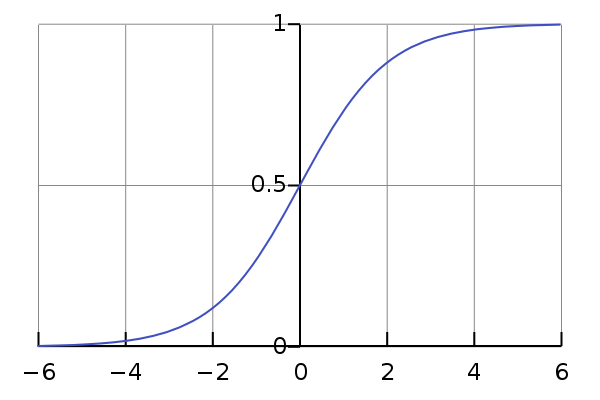
\includegraphics[scale = 0.4]{Logistic-curve.png}
  \caption{Sigmoid function}
\end{figure}

\subsubsection{Whats sigmoid function?}
A sigmoid function refers to a mathematical function that is bounded, differentiable, and defined for all real
input values. It exhibits a characteristic "S"-shaped curve and has a non-negative derivative at every point.
It is important to note that the terms "sigmoid function" and "sigmoid curve" refer to the same mathematical
object. which is defined by the formula:
\[
S(x) = \frac{1}{1 + e^{-x}} = \frac{e^x}{e^x + 1} = 1 - S(-x)
\]
This expression provides us with the following information.
\[
x \rightarrow \infty \quad \implies \quad S(x) = \frac{1}{1 + e^{-x}} \rightarrow 1
\]
\[
x \rightarrow  - \infty \quad \implies \quad S(x) = \frac{1}{1 + e^{-x}} \rightarrow 0
\]
Which fits perfectly as a solution to our problem.
\subsection{Using MSE for classification}
This concept may not be intuitively clear, but it effectively measures the error of the neuron.
Therefore, the function $MSE$ designed for classification tasks should resemble the following form.
\[
MSE(\vec{w}) = \frac{1}{n} \cdot \sum_{t = 1}^{n}(y_t - \frac{1}{1 + e^{-(\vec{x}_t \cdot \vec{w})}})^2
\]
Building upon the previous concept of gradient descent, we can derive these formulas. I understand that
this may seem challenging, but studying calculus and revisiting these ideas will enable you to comprehend
how these algorithms function.\\
Again first lets define our $u_t$

\[
u_t = y_t - \frac{1}{1 + e^{-(\vec{x}_t \cdot \vec{w})}} = y_t - \frac{1}{1 + e^{-(\sum_{i = 1}^m x_{t, i} \cdot w_i)}}
= y_t - \frac{1}{1 + e^{-x_{t, 1} \cdot w_1} \cdots e^{-x_{t, m} \cdot w_m}}
\]

Finding the derivative of $w_i$ in this case is not straightforward due to the presence of a fraction and
the Euler exponential. However, by following the fundamental rules of derivatives, we can tackle this challenge.

\[
f(x) = \frac{g(x)}{h(x)}
\]

\[
\frac{d(f(x))}{dx} = \frac{\frac{d(g(x))}{dx} \cdot h(x) - \frac{d(h(x))}{dx} \cdot g(x)}{h^2(x)}
\]

\[
f(x) = c_1 \cdot e^{c_2 \cdot x}
\]

\[
\frac{d(f(x))}{dx} = c_1 \cdot c_2 \cdot e^{c_2 \cdot x}
\]

Folling those rules we arrive with this idea of the derivate $u_t$ of $w_i$, lets view.
\[
u_t(\vec{w}) = \frac{g(\vec{w})}{h(\vec{w})}
\]

\[
g(\vec{w}) = 1
\]

\[
h(\vec{w}) = 1 + e^{-(\vec{x}_t \cdot \vec{w})} = 1 + e^{-(\sum_{i = 1}^m x_{t, i} \cdot w_i)}
= 1 + e^{-x_{t, 1} \cdot w_1} \cdots e^{-x_{t, m} \cdot w_m}
\]

\[
\frac{\partial g(\vec{w})}{\partial w_i} = 0
\]

\[
\frac{\partial h(\vec{w})}{\partial w_i}
= -x_{t, i} \cdot e^{-x_{t, 1} \cdot w_1} \cdots e^{-x_{t, i} \cdot w_i} \cdots e^{-x_{t, m} \cdot w_m}
\]

\[
\frac{\partial u_t}{\partial w_i} =
\frac{- (-x_{t, i} \cdot e^{-x_{t, 1} \cdot w_1} \cdots e^{-x_{t, i} \cdot w_i} \cdots e^{-x_{t, m} \cdot w_m})}
     {(1 + e^{-x_{t, 1} \cdot w_1} \cdots e^{-x_{t, m} \cdot w_m})^2}
     \]
     \[
     = \frac{x_{t, i} \cdot e^{-x_{t, 1} \cdot w_1} \cdots e^{-x_{t, i} \cdot w_i} \cdots e^{-x_{t, m} \cdot w_m}}
     {1 + 2e^{-x_{t, 1} \cdot w_1} \cdots e^{-x_{t, m} \cdot w_m} + e^{-2 \cdot x_{t, 1} \cdot w_1} \cdots e^{-2 \cdot x_{t, m} \cdot w_m}}
\]
I understand that these types of derivatives can be challenging to grasp, but by studying
differential calculus, you will be able to overcome the difficulties and comprehend them.

\[
\frac{\partial u_t}{\partial w_i} =
\frac{x_{t, i} \cdot e^{- \vec{x}_t \cdot \vec{w}}}
     {(1 + e^{- \vec{x}_t \cdot \vec{w}})^2}
\]

Continuing with the chain rule, we can arrive at these expressions.
\[
\frac{\partial MSE}{\partial w_i} = \frac{1}{n} \cdot (\frac{\partial u_1^2}{\partial u_1} \cdot
\frac{u_1}{w_i} + \cdots + \frac{\partial u_n^2}{\partial u_n} \cdot \frac{\partial u_n}{\partial w_i})
\]


\[
\frac{\partial MSE}{\partial w_i} = \frac{1}{n} \cdot (2 \cdot u_1 \cdot
\frac{x_{1, i} \cdot e^{- \vec{x}_1 \cdot \vec{w}}}{(1 + e^{- \vec{x}_1 \cdot \vec{w}})^2}
+ \cdots +
2 \cdot u_n \cdot
\frac{x_{n, i} \cdot e^{- \vec{x}_n \cdot \vec{w}}}{(1 + e^{- \vec{x}_n \cdot \vec{w}})^2}
\]

\[
\frac{\partial MSE}{\partial w_i} = \frac{2}{n} \cdot (
(y_1 - \frac{1}{1 + e^{-(\vec{x}_1 \cdot \vec{w})}}) \cdot
\frac{x_{1, i} \cdot e^{- \vec{x}_1 \cdot \vec{w}}}{(1 + e^{- \vec{x}_1 \cdot \vec{w}})^2}
+ \cdots +
(y_n - \frac{1}{1 + e^{-(\vec{x}_n \cdot \vec{w})}}) \cdot
\frac{x_{n, i} \cdot e^{- \vec{x}_n \cdot \vec{w}}}{(1 + e^{- \vec{x}_n \cdot \vec{w}})^2}
)
\]


\[
\frac{\partial MSE}{\partial w_i} = \frac{2}{n} \cdot \sum_{t = 1}^n
(y_t - \frac{1}{1 + e^{-\vec{x}_t \cdot \vec{w}}}) \cdot
\frac{x_{t, i} \cdot e^{- \vec{x}_t \cdot \vec{w}}}{(1 + e^{- \vec{x}_t \cdot \vec{w}})^2}
\]

And that's it! By finding the gradient, we can now implement the gradient descent algorithm
for neuron classification.
\[
\nabla MSE(\vec{w}) =
\begin{bmatrix} \frac{\partial MSE}{\partial w_1}(\vec{w})
  \\ \vdots
  \\ \frac{\partial MSE}{\partial w_m}(\vec{w})
\end{bmatrix} =
\begin{bmatrix} \frac{2}{n} \cdot \sum_{t = 1}^n
  (y_t - \frac{1}{1 + e^{-(\vec{x}_t \cdot \vec{w})}}) \cdot
  \frac{x_{t, 1} \cdot e^{- \vec{x}_t \cdot \vec{w}}}{(1 + e^{- \vec{x}_t \cdot \vec{w}})^2}
  \\ \vdots
  \\ \frac{2}{n} \cdot \sum_{t = 1}^n  (y_t - \frac{1}{1 + e^{-(\vec{x}_t \cdot \vec{w})}}) \cdot
  \frac{x_{t, m} \cdot e^{- \vec{x}_t \cdot \vec{w}}}{(1 + e^{- \vec{x}_t \cdot \vec{w}})^2}
\end{bmatrix}
\]

\[
\vec{w}_{k + 1} = \vec{w}_{k} + \gamma \cdot \nabla MSE(\vec{w}_k)
\]

\subsubsection{The Origin of the Name "Gradient Descent"}
Essentially, the name "gradient descent" derives from the concept of descending along the gradient of a
parabolic graph, as demonstrated earlier. As the weights are updated, they gradually move downwards,
resembling a descent. The following illustration depicts this idea, with each node representing a weight update.
\begin{figure}[H]
  \centering
  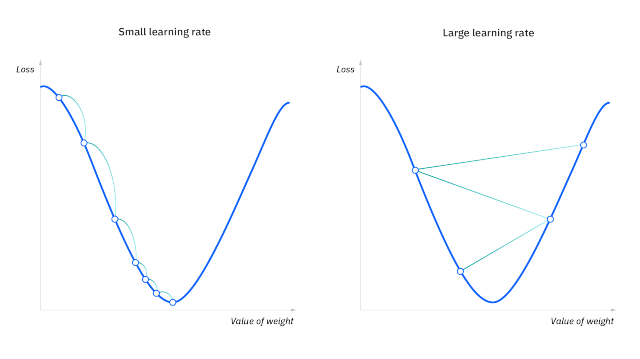
\includegraphics[scale = 0.7]{gradient_descent.png}
  \caption{Gradient descent}
\end{figure}

\section{From algorithm to code}
In this section, we will learn how to code the new optimized learning algorithm for both prediction
and classification neurons, then. When it comes to dealing with derivatives, there are different approaches
available.
One common method is to approximate the derivatives of a function using numerical techniques such as
finite differences. This method is relatively straightforward and relies on the concept of derivatives.
In the case of a multivariable function, the approximation would look something like this.


\[
\frac{\partial (f(\vec{x}))}{\partial x_i} \approx \frac{f(x_1, \cdots, x_i + h, \cdots, x_n) -
  f(x_1, \cdots, x_i, \cdots, x_n)}{h}
\]

Here, the parameter $h$ is not constrained by any specific limit. It represents your choice of
approximation, allowing you to determine the desired level of precision for the approximation.\\

However, in our case, we have derived and arrived at useful mathematical expressions
for both prediction and classification in the previous section so we are going to use it.

\subsection{Coding the Optimized Learning Algorithm for the Prediction Neuron}
So the algorithm doesn't change much. Let's begin by coding our $MSE(\vec{w})$ function to measure
the error of our model.
\[
MSE(\vec{w}) = \frac{1}{n} \cdot \sum_{t = 1}^ny_t - \vec{x}_t \cdot \vec{w}
\]

The code translation of this would look something like the following.
\begin{verbatim}
diffs = 0.0
for (t = 0, t < n, t++)
    res = 0.0
    for (i = 0, i < input[t].size(), i++)
        res += (inputst[t][i] * weigths[i])
    diffs += pow(outputs[t] - res, 2.0)  // Compute the square

return  diffs / n
\end{verbatim}
With this code written as a function, we now have the ability to measure the performance of our model.
As for the learning algnnorithm, as I mentioned earlier, the new algorithm for updating our weights doesn't
need to change much. You only need to keep in mind this expression.
\[
\frac{\partial MSE}{\partial w_i} = \frac{2}{n} \cdot \sum_{t = 1}^n(y_t - \vec{x}_t \cdot \vec{w}) \cdot x_{t, i}
\]
First define your number of epochs, and learning rate which is gamma $\gamma$.
\begin{verbatim}
gamma = 0.1
nepochs = 100
\end{verbatim}
Now, let's proceed with coding the algorithm. Since this algorithm iteratively works by summing values,
there are multiple approaches to achieve the same result. Hence, the following implementation is not the
only way to do it.
\begin{verbatim}
for (e = 0, e < nepochs, e++)
    errors[n] = {0.0}
    // First compued the whole errors
    for (t = 0, t < n, t++)
        res = 0.0
        for (i = 0, i < input[t].size(), i++)
            res += inputst[t][i] * weigths[i]
        errors[t] = outputs[t] - res

    // After update all the weights
    for (i = 0, i < weights.size(), i++)
        update = 0.0
        for (t = 0, t < n, t++)
            update += errors[t] * input[t][i]
        weights[i] += (2 / n) * gamma * update
\end{verbatim}

\subsection{Coding the Optimized Learning Algorithm for the Classification Neuron}
Now, let's begin implementing the algorithm for the classification neuron. The first step is to code
the sigmoid function activation, which is essential for our computations.
\begin{verbatim}
function activation(x)
         return 1 / (1 + exp(- x))
end function
\end{verbatim}
ost programming languages have a built-in function called $exp$ that represents the exponential function $e^x$.
With this function, we can proceed to code our own $MSE$ function to assess the accuracy of our model.
\[
MSE(\vec{w}) = \frac{1}{n} \cdot \sum_{t = 1}^{n}(y_t - \frac{1}{1 + e^{-(\vec{x}_t \cdot \vec{w})}})^2
\]
\begin{verbatim}
diffs = 0.0
for (t = 0, t < n, t++)
    res = 0.0
    for (i = 0, i < input[t].size(), i++)
        res += inputst[t][i] * weigths[i]
    diffs += pow(outputs[t] - activation(res), 2.0) // notice that I call activation

return  diffs / n
\end{verbatim}
The learning algorithm for the classification neuron is slightly different, as we introduce the sigmoid
function and incorporate new expressions into it. As a result, the code would look like the following,
but just try to follow this expression.
\[
\frac{\partial MSE}{\partial w_i} = \frac{2}{n} \cdot \sum_{t = 1}^n
(y_t - \frac{1}{1 + e^{-\vec{x}_t \cdot \vec{w}}}) \cdot
\frac{x_{t, i} \cdot e^{- \vec{x}_t \cdot \vec{w}}}{(1 + e^{- \vec{x}_t \cdot \vec{w}})^2}
\]

I hope you have understood this code. If you find it challenging to comprehend, I recommend trying to write
your own algorithm and then revisiting this code. My approach aims to minimize computations for improved
efficiency, and I believe there is room for further optimization.
\begin{verbatim}
for (e = 0, e < nepochs, e++)
    errors[n] = {0.0}
    // Notice that I'm creating this array to save computations
    results[n] = {0.0}
    // First compued the whole errors
    for (t = 0, t < n, t++)
        res = 0.0
        for (i = 0, i < input[t].size(), i++)
            res += inputs[t][i] * weigths[i]
        results[t] = res
        errors[t] = outputs[t] - activation(res)

    // After update all the weights
    for (i = 0, i < weights.size(), i++)
        update = 0.0
        for (t = 0, t < n, t++)
            update += errors[t] * pow(activation(results[t]), 2.0)
                      * inputs[t][i] * exp(- results[t])
        weights[i] += (2 / n) * gamma * update
\end{verbatim}
You might be wondering about the feed-forward code, but I believe it is unnecessary to
show it here since it is practically the same code we have written in the previous chapter.
\section{Examples}
I have created a Fortran module that supports both types of neurons. After implementing the module,
I have organized illustrative examples that you can explore in the following link:
\href{https://github.com/alecksandr26/fortran-ml/tree/main/examples}{examples}.
Feel free to check
them out while you continue reading this section.
\subsection{Fortran module for both neurons}
As mentioned earlier, I designed the module to support both types of neurons, aiming for a more generalized
approach. This allows for code reusability across various problem domains. By adopting this design, we can
leverage the module for a wide range of applications.

\begin{lstlisting}

\end{lstlisting}






\Chapter{Artificial Neural Networks}{The path to archive real intelligence}


\section{Unleashing the Power of Artificial Neural Networks (ANNs)}
In the previous chapters, we have discussed a key challenge encountered in neurons: the linearity of problems.
In some cases, problems are not linear and cannot be easily separated or solved using linear regression
techniques alone. To address this, we introduced the idea of using multiple neurons and now the time has
come to delve into building our first neural network from scratch. It's important to note that neural
networks have their own peculiarities and understanding linear algebra, including concepts such as matrix
construction and solving linear systems, will greatly aid in comprehending how these models truly function.
I highly recommend studying linear algebra to ensure a solid foundation for the upcoming explanations.\\

This approach of ANNs
is inspired by how our brain cells works. Our brain consists of billions of interconnected
neurons, and drawing from this concept, we can create
several artificial neurons and connect their outputs to inputs.
By adjusting the weights or parameters of the neural network, we can observe if it can produce valuable outputs.
In essence, we are attempting to mimic the functioning of the brain using artificial neural networks (ANNs).

\begin{figure}[H]
  \centering
  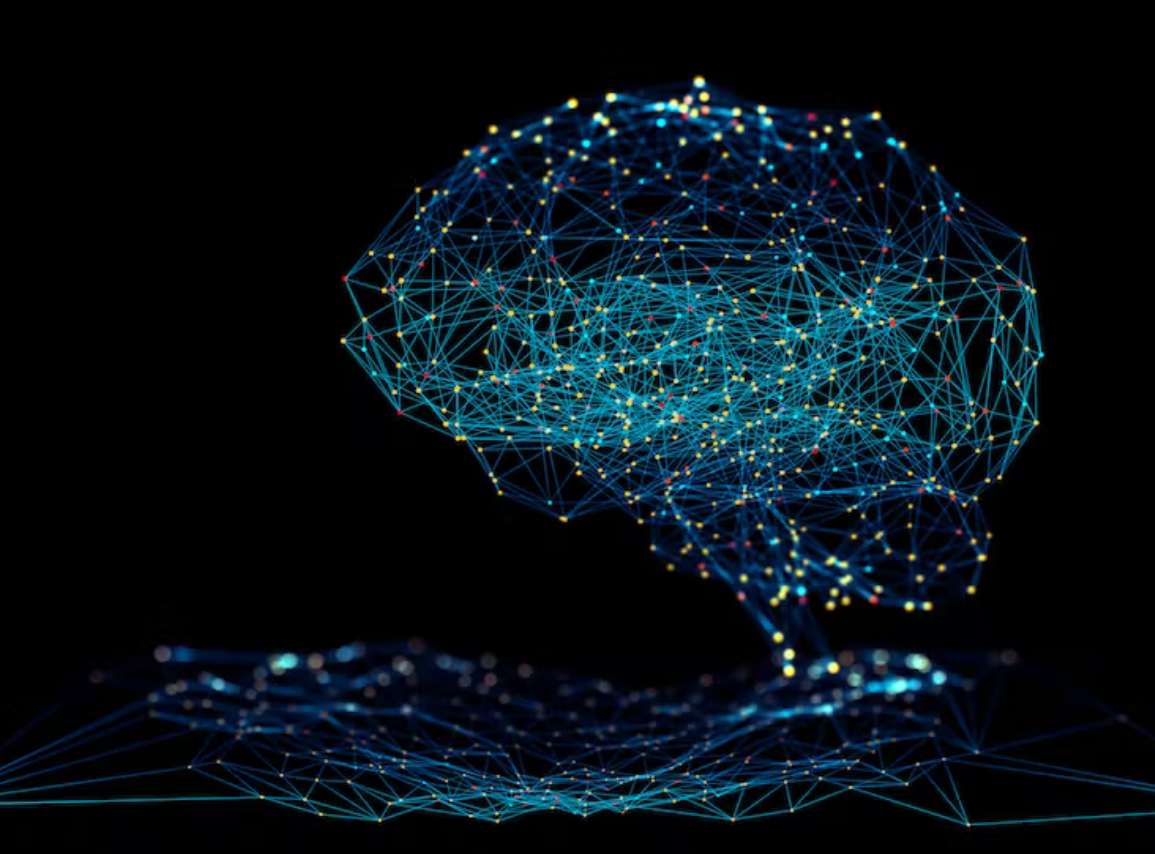
\includegraphics[scale = 0.3]{neural_networks.png}
  \caption{The brain cells}
\end{figure}
Next, let's examine the components of an Artificial
Neural Network to gain a better understanding of how they operate.
\subsection{Components of an Artificial Neural Network}
\begin{figure}[H]
  \centering
  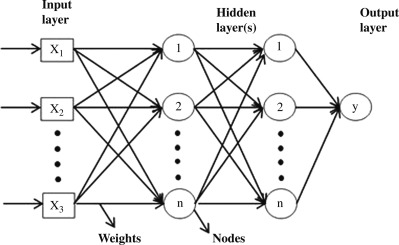
\includegraphics[scale = 1.3]{nerual_network.jpg}
  \caption{The neural network}
\end{figure}
\begin{itemize}
\item \textbf{Input Layer}: The input layer of a neural network may not always consist of artificial neurons.
  In certain cases, such as when combining multiple neural networks, the input can be sourced from the output
  of another neural network. However, in the context of a simple neural network, the input layer is represented
  by an array or vector that serves as the input data for the network.
  
\item \textbf{Hidden Layer}: The hidden layers of a neural network consist of groups of artificial neurons
  arranged vertically. Each hidden layer receives inputs and produces outputs. The term "hidden" refers to
  the fact that these layers are not directly observable from the network's input or output. The connections
  between the artificial neurons enable the flow of information and allow for complex computations to take
  place within the hidden layers.
  
\item \textbf{Output Layer}: The output layer, similar to the hidden layers, is composed of multiple neurons.
  In the previous image, only one node is shown for simplicity, but in reality, a neural network can have
  multiple output neurons, especially for classifying more complex patterns or performing multiple tasks
  simultaneously. The output layer receives the outputs from the hidden layers and performs the final
  computations to generate the desired output or prediction.
\end{itemize}
\subsection{The XOR Problem}
One of the limitations of the perceptron is its inability to solve the XOR logic gate problem, which is
not linearly separable. This means that a single neuron cannot accurately classify the XOR inputs.
I conducted an experiment to test this, and the results clearly show that the perceptron fails to converge
when trained on the XOR problem.
\begin{verbatim}
MSE: 0.250000
1, 1: 0.500000
0, 1: 0.500000
1, 0: 0.500000
0, 0: 0.500000
 Weights:    0.00000000       0.00000000       0.00000000    
\end{verbatim}
The mean squared error (MSE), which is our cost function, gives us an error of $0.25$, which is the lowest
achievable error. However, this result is quite peculiar because in computer architectures, an XOR logic
gate is typically implemented using other logic gates.
\begin{figure}[H]
  \centering
  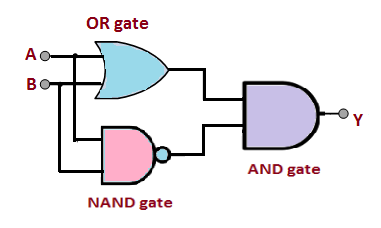
\includegraphics[scale = 1.0]{xor-equivalent-circuit.png}
  \caption{XOR equivalent circuit}
\end{figure}
As you can see, this illustrates the fundamental idea of neural networks: using multiple neurons to achieve
more complex and precise computations. The following diagram represents the XOR neural network,
which demonstrates the
power of combining neurons to solve non-linearly separable problems.


\begin{center}
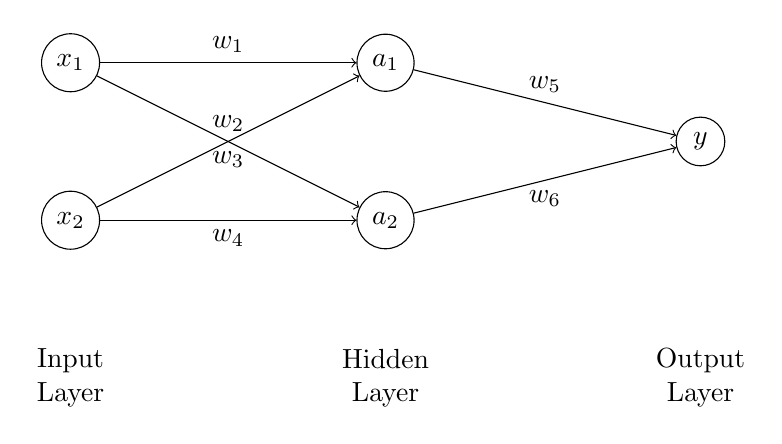
\begin{tikzpicture}[scale=2.0]
  % Input layer
  \node[circle, draw] (input1) at (0,0) {$x_1$};
  \node[circle, draw] (input2) at (0,-1) {$x_2$};

  % Hidden layer
  \node[circle, draw] (hidden1) at (2,0) {$a_1$};
  \node[circle, draw] (hidden2) at (2,-1) {$a_2$};

  % Output layer
  \node[circle, draw] (output) at (4, -0.5) {$y$};

  % Edges with weights
  \draw[->] (input1) -- node[midway, above] {$w_1$} (hidden1);
  \draw[->] (input2) -- node[midway, above] {$w_2$} (hidden1);
  \draw[->] (input1) -- node[midway, below] {$w_3$} (hidden2);
  \draw[->] (input2) -- node[midway, below] {$w_4$} (hidden2);
  \draw[->] (hidden1) -- node[midway, above] {$w_5$} (output);
  \draw[->] (hidden2) -- node[midway, below] {$w_6$} (output);

  % Labels
  \node[align = center] at (0, -2) {Input\\Layer};
  \node[align = center] at (2, -2) {Hidden\\Layer};
  \node[align = center] at (4, -2) {Output\\Layer};
\end{tikzpicture}
\end{center}

In total, this network architecture consists of three artificial neurons. Let's dive into the mathematical
calculations for these neurons. We can consider $a_1$ and $a_2$ as the result variables obtained from the
computations of those neurons. The mathematical expression utilizing the sigmoid function for these
computations is as follows.
\[
a_1 = \sigma(b_1 + x_1 \cdot w_1 + x_2 \cdot w_2)
\]
\[
a_2 = \sigma(b_2 + x_1 \cdot w_3 + x_2 \cdot w_4)
\]
If you study linear algebra, as mentioned at the beginning of this chapter, you will start noticing a pattern,
right? To be more precise, the expressions shown above exhibit a matrix multiplication. Let's take a closer
look: We can interpret our input vector $\vec{x} = \{x_1, x_2\}$ as a matrix $X$.
\[
X = \begin{bmatrix} x_1 \\ x_2 \end{bmatrix}
\]
And similarly, with our weights, in the previous chapter we saw our bias as part of the weight vector
$\vec{w} = \{b, w_2, \cdots, w_n\}$. However, for today's explanation, we will separate the bias
from the weights to simplify the equations and expressions.
\[
W_1 = \begin{bmatrix} w_1 & w_3 \\ w_2 & w_4 \end{bmatrix}
\quad
B_1 = \begin{bmatrix} b_1 \\ b_2 \end{bmatrix}
\]
And we can also consider $a_1$ and $a_2$ as elements of a result matrix. In matrix form, we can represent
them as:

\[
A_1 = \begin{bmatrix} a_1 \\ a_2 \end{bmatrix}
\]

And essentially, with these matrices, we can abstract the above computations as simple matrix
multiplications followed by passing the result through an activation function. Take a look:
\[
A_1^T = \sigma(X^T \cdot W_1 + B_1^T) = \begin{bmatrix} a_1 & a_2 \end{bmatrix}
\]

when we use $X^T$, it refers to the transpose matrix of $X$, which means rearranging the components of the
matrix into a different order. This allows us to perform operations such as matrix multiplication
between $X^T$ and another matrix, taking into account the rearranged structure.
\[
X = \begin{bmatrix} x_1 \\ x_2 \end{bmatrix}
\]
\[
X^T = \begin{bmatrix} x_1 & x_2 \end{bmatrix}
\]
And this is not the only approach to performing these computations. Another way is to consider the transpose
of $W$ instead of $X$. Both approaches yield the same results. I mention this to avoid confusion if you come
across different explanations while learning about these concepts elsewhere.
\[
A_1 = \sigma(W_1^T \cdot X + B_1) = \begin{bmatrix} a_1 \\ a_2 \end{bmatrix}
\quad \quad A_1 = \sigma(\begin{bmatrix} w_1 & w_2 \\ w_3 & w_4 \end{bmatrix} \cdot
\begin{bmatrix} x_1 \\ x_2 \end{bmatrix} + \begin{bmatrix} b_1 \\ b_2 \end{bmatrix}) =
\begin{bmatrix} a_1 \\ a_2 \end{bmatrix}
\]
It is important to note that the order of matrix multiplication determines the structure of the resulting
matrix. In the context of neural networks, this concept becomes significant. After obtaining the matrix $H_1$
from the previous computations, it is used as input for the next layer. This process of passing outputs from
one layer to another forms the basis of the feedforward operation in a neural network. As you can see, it is
a sequential flow of matrix operations.
\[
W_2 = \begin{bmatrix} w_5 \\ w_6 \end{bmatrix} \quad
Y = \sigma(W_2^T\cdot A_1 + B_2) = \begin{bmatrix} y \end{bmatrix} = y
\]

At the end, a simple number can be thought of as a matrix with a single component, represented as $Y = [y] = y$.
This approach allows us to treat scalar values as matrices, ensuring consistency and compatibility with matrix
operations in neural networks. As you can see, it is not overly complicated from a matrix perspective.
\subsection{Understanding Feedforward in Artificial Neural Networks}
Feedforward is a commonly used term in artificial intelligence, referring to the process of taking an input and
passing it through the layers of complexity to obtain an output. By abstracting the artificial neuron layers
to matrices, we can simplify the computation of each layer. In essence, we can think of this process as follows:
\[
A_l = f(W_l^T \cdot A_{l - 1} + B_l) = \begin{bmatrix} a_{1}^l \\ \vdots \\ a_{n}^l \end{bmatrix}
\]
In the equation, $A_{l-1}$ represents the output from the previous layer. We observe that $A_{l-1}$ has the same
number of rows as the number of columns in $W_l^T$. This is denoted by the outputs $a_{1}^l, \ldots, a_{n}^l$,
where $l$ represents the current layer. This notation enables us to distinguish between the various outputs
$a$ across the network. Additionally, $W_l$ and $B_l$ correspond to the weight matrix and bias vector of the
current layer, respectively, while $f$ represents the activation function.
\[
W_l = \begin{bmatrix} w_{1, 1}^l & w_{1, 2}^l & \cdots & w_{1, n}^l \\
  w_{2, 1}^l & w_{2, 2}^l & \cdots & w_{2, n}^l \\
  \vdots & \vdots & \cdots & \vdots \\
  w_{m, 1}^l & w_{m, 2}^l & \cdots & w_{m, n}^l
\end{bmatrix}
\quad\quad B_l = \begin{bmatrix} b_{1}^l \\ b_{2}^l \\ \vdots \\ b_{n}^l \end{bmatrix}
\]
In this context, $n$ refers to the number of neurons in the current layer, and $m$ represents
the number of weights associated with each neuron or the number of neurons in the previous layer.
The subscript $l$ indicates the current layer. Additionally, the transpose of the weight matrix can be
represented as follows:
\[
W_l^T = \begin{bmatrix} w_{1, 1}^l & w_{2, 1}^l & \cdots & w_{m, 1}^l \\
  w_{1, 2}^l & w_{2, 2}^l & \cdots & w_{m, 2}^l \\
  \vdots & \vdots & \cdots & \vdots \\
  w_{1, n}^l & w_{2, n}^l & \cdots & w_{m, n}^l
\end{bmatrix}
\]
At the end, the structure of the initial $W_l$ can be simplified to avoid complexity. There isn't just one
way to approach these computations; it depends on the perspective you choose and what you consider to be the
most optimal method.
\[
W_l = \begin{bmatrix} w_{1, 1}^l & w_{1, 2}^l & \cdots & w_{1, m}^l \\
  w_{2, 1}^l & w_{2, 2}^l & \cdots & w_{2, m}^l \\
  \vdots & \vdots & \cdots & \vdots \\
  w_{n, 1}^l & w_{n, 2}^l & \cdots & w_{n, m}^l
\end{bmatrix}
\]

\[
A_l = f(W_l \cdot A_{l - 1} + B_l) = \begin{bmatrix} a_{1}^l \\ \vdots \\ a_{n}^l \end{bmatrix}
\]

Just keep in mind the variables $m$, which represent the number of weights or the number of neurons from the
previous layer, and the variable $n$, which refers to the number of neurons in the current layer.
When discussing the algorithmic process, we repeat this computation for all $l$ layers. So, you can think of
the first layer as follows:
\[
A_1 = f(W_1 \cdot X + B_1) = \begin{bmatrix} a_{1}^1 \\ \vdots \\ a_{n}^1 \end{bmatrix}
\]
Then, we can consider the last layer as the output layer $k$ and it should be something as follows:
\[
Y = A_k =  f(W_k \cdot A_{k - 1} + B_k) 
= \begin{bmatrix} a_{1}^k \\ \vdots \\ a_{n}^k \end{bmatrix}
= \begin{bmatrix} y_{1} \\ \vdots \\ y_{n} \end{bmatrix}
\]
Where $k$ is the last layer from this system.
I understand that there is a lot of notation involved, but it is crucial to have a clear understanding of all
the variables and their meanings. The feedforward process can be seen as a composition of multiple functions,
where each layer's output serves as the input for the next layer. It is important to ensure that you can
comprehend this expression and its implications.
\[
Y = f(W_k \cdot f(
W_{k - 1} \cdot f(\cdots f(W_{1} \cdot X + B_1) \cdots) + B_{k - 1}
) + B_k) = \begin{bmatrix} y_1 \\ \vdots \\ y_{r} \end{bmatrix}
\quad \quad | \quad \quad X = \begin{bmatrix} x_1 \\ \vdots \\ x_{d} \end{bmatrix}
\]

Rather than treating it as a basic function, it is crucial to recognize that an artificial
neural network operates
as a nonlinear system. Unlike the perceptron, which processes individual inputs, a neural network receives
a column vector or matrix $X$ and generates an output column vector or matrix $Y$.

\[
\mathcal{N}: \quad \mathbb{R}^d \quad  \rightarrow \quad \mathbb{R}^r \quad | \quad d,r \in \mathbb{N} 
\]
Where $\mathcal{N}$ represent the artificial neural network.
Mathematically speaking, artificial neural networks can be understood as linear transformations or mappings.

\subsection{Intuition Behind Neural Networks}
The underlying concept behind these expressions and neural networks is that each layer creates an
abstraction of the input data. Whether it's detecting patterns for linear separability or regression,
each layer captures and quantifies the presence of these patterns. This information is then passed on
to the next layer of neurons, and this process continues until reaching the output layer, which ultimately
makes a decision or classification.

To illustrate this concept, consider a child learning to identify clocks. At the initial stage, the child
recognizes that a clock is a circular object, representing the first level of abstraction. As the child
progresses, they discover that clocks have numbers and an arrow, representing a second layer of abstraction.
Eventually in the last layer, the child grasps the concept of telling time, which emerges from these layers
of abstractions. This is analogous to how a neural network understands and learns.

by each individual neuron within these layers remains somewhat mysterious due to the complexity of the
underlying mathematical derivatives, which we will discuss in the next section. The key point here is that
the hidden layers operate at a highly abstract level, and through a process of convergence, the network as a
whole learns to perform seemingly magical computations. This is the unleashing power of neural networks,
where these parameters or weights enable the network to abstract and classify more complex concepts and ideas.

\section{How to train an Artificial Neural Network?}
As I mentioned earlier, training a neural network is not an easy task. In fact, the concept of
ANNs is not new and dates back to the 1960s. However, during that time, the main challenges were
related to computing power and the lack of understanding of effective training methods.

Let's break it down step by step. First, we need to define a cost function that quantifies the error of
our model.
However, this task can be somewhat challenging starting with
the fact that a neural network can have multiple outputs.

\[
Y = \begin{bmatrix} y_1 \\ \vdots \\ y_n \end{bmatrix}
\]

Therefore, for each output generated by our neural network, there should be a corresponding desired output.
\[
Y_t = \begin{bmatrix} y_{1}^t \\ \vdots \\ y_{n}^t \end{bmatrix}
\]

Here, $t$ represents the current training example for each input matrix $X_t$.
From this, we can infer that for each $y_{i}^t$, we can calculate an error measurement.
\[
E =
\begin{bmatrix}
  \frac{1}{N} \cdot \sum_{t = 1}^{N}(y^t_{1} - \overset{\sim}{y_{1}^t})^2 \\ \vdots \\
  \frac{1}{N} \cdot \sum_{t = 1}^{N}(y^t_{n} - \overset{\sim}{y_{n}^t})^2
\end{bmatrix}
\]

Here, $\overset{\sim}{y_{1}^t}$
represents the predicted output from the neural network. We can interpret the matrix or vector
of errors by summing up all the individual errors and $N$ the amount of
the dataset $\mathbb{D}$. Since this matrix has only one column, we
can simplify the calculation by using a single summation. This expression, often referred to as
the cost function or loss function, provides a measure of the error generated by the neural network.

\[
C = \sum_{i = 1}^{n} E_{i, 1}
\]

Indeed, all the weights in our neural network have an impact on the error expression. This complexity is
what makes training a neural network challenging. It becomes difficult to find an expression that guides
us in updating the weights effectively. Just imagine the task of deriving an expression to update the
weights—it's quite daunting.
\[
\frac{\partial C}{\partial w_{i, j}^l} = ?
\]

However, it is important to remember that the output $Y$ of a neural network is a composition of numerous
activation functions. This complexity makes it extremely challenging to derive mathematical expressions for
computing the partial derivatives with respect to each weight. It can feel overwhelming due to the sheer number
of computations involved.

\[
Y = f(W_k \cdot f(
W_{k - 1} \cdot f(\cdots f(W_{1} \cdot X + B_1) \cdots) + B_{k - 1}
) + B_k) = \begin{bmatrix} y_1 \\ \vdots \\ y_{n} \end{bmatrix}
\]

For small neural networks, it is possible to derive general formulas for updating each weight using the
chain rule. However, this approach becomes impractical and non-scalable for larger networks due to the
complexities involved in programming and implementation. As an alternative, we can use finite differences
to approximate the derivatives. Although this introduces some bias in the precision of our calculations,
the main challenge lies in the computational cost. As the neural network grows in size, both in terms of
layers and weights, the time required to compute the approximate derivatives increases exponentially.
Despite this drawback, using finite differences allows us to address the problem by brute-forcing each
individual derivative.\\

\subsection{Brute forcing learning algorithm}
The approach of finite differences involves choosing a small value for $h > 0$ and adopting a
computational method. In this scenario, we consider our cost function as $f$ and $x_i$ as the weight
for which we want to approximate its rate of change with respect to $C$.
\[
\frac{\partial (f(\vec{x}))}{\partial x_i} \approx \frac{f(x_1, \cdots, x_i + h, \cdots, x_n) -
  f(x_1, \cdots, x_i, \cdots, x_n)}{h}
\]
Implementing this approach requires computing the actual cost $C$ using the current weights,
which in turn necessitates calculating all the outputs for the given dataset.
\[
C = \sum_{i = 1}^{n} E_{i, 1}
\quad | \quad
E =
\begin{bmatrix}
  \frac{1}{N} \cdot \sum_{t = 1}^{N}(y^t_{1} - \overset{\sim}{y_{1}^t})^2 \\ \vdots \\
  \frac{1}{N} \cdot \sum_{t = 1}^{N}(y^t_{n} - \overset{\sim}{y_{n}^t})^2
\end{bmatrix}
\quad | \quad \mathcal{N}: X_t \rightarrow Y_t
\quad \forall X_t \in \mathbb{D}
\]
In this case, $\mathcal{N}$ represents our neural network, which maps input $X_t$ to output $Y_t$. Therefore,
to obtain our desired cost function, we must compute all the outputs for the entire dataset
$\mathbb{D}$. Once we have the actual cost, we can proceed to modify the specific weight $w_{i, j}^l$
using a small value of $h$.
\[
w_{i, j}^l + h = \overset{\sim}{w_{i, j}^l}
\]
After making a small change to the network, we need to compute the modified version of $C$,
denoted as $\overset{\sim}{C}$. This implies that we must recompute all the outputs for the entire dataset again.
\[
\overset{\sim}{C}= \sum_{i = 1}^{n} E_{i, 1}
\quad | \quad E =
\begin{bmatrix}
  \frac{1}{N} \cdot \sum_{t = 1}^{N}(y^t_{1} - \overset{\sim}{y_{1}^t})^2 \\ \vdots \\
  \frac{1}{N} \cdot \sum_{t = 1}^{N}(y^t_{n} - \overset{\sim}{y_{n}^t})^2
\end{bmatrix}\quad | \quad \mathcal{N}: X_t \rightarrow Y_t
\quad \forall (X_t,Y_t) \in \mathbb{D}
\]

I don't know about you, but computing matrix multiplications can be quite time-consuming.
After going through all these calculations, we finally obtain an approximation of the rate of change.

\[
\frac{\partial C}{\partial w_{i, j}^l} \approx \frac{\overset{\sim}{C} - C}{h}
\]

Yes, we have finally completed the process. Now, we just need to repeat this entire process for each
weight $w_{i, j}^l$ within the neuron, then for each layer $l$ until you reach $k$ layer. However,
this approach is highly inefficient and computationally demanding. In fact, back in the 1960s, with the
limited computing power available, it was not feasible to perform these calculations. Even today, with
more powerful computers, performing deep learning tasks using this algorithm on a regular desktop computer
is simply impractical.\\

Throughout this chapter, we have not delved into any deep learning ANNs.
However, in the next chapter,
we will explore how to address this issue and optimize the learning algorithm for ANNs.
We will introduce the Back Propagation algorithm, which builds upon the fundamental principles of
gradient descent and provides a solution for adjusting the weights without relying on brute force methods.

\section{The Convergence Proof of ANNs}

\section{Coding Our First Neural Network}



\chapter{References}
\begin{itemize}
\item Zieba, J., PhD. (2022, December 16). How Do Neurons Work? The Scientist Magazine®.
  \url{https://www.the-scientist.com/university/brush-up-how-do-neurons-work-70839}
\item Action potentials and synapses. (2017, November 9). Queensland Brain Institute - University
  of Queensland.
  \url{https://qbi.uq.edu.au/brain-basics/brain/brain-physiology/action-potentials-and-synapses}
\item Perceptrons. (n.d.). \url{https://www.w3schools.com/ai/ai_perceptrons.asp}
\item Perceptron in Machine Learning - Javatpoint. (n.d.). www.javatpoint.com.
  \url{https://www.javatpoint.com/perceptron-in-machine-learning}
\item Training a Perceptron. (n.d.). \url{https://www.w3schools.com/ai/ai_training.asp}
\item Desmedt, S. (2019, May 12). The Math behind Neural Networks: Part 1 - The Rosenblatt Perceptron.
  CodeProject.
  \href{https://www.codeproject.com/Articles/4047091/The-Math-behind-Neural-Networks-Part-1-The-Rosenbl}{
    url}
\item Wikipedia contributors. (2023, March 21). Dot product. Wikipedia.
  \url{https://en.wikipedia.org/wiki/Dot_product}
\item Kilian Weinberger. (2018, July 9). Lecture 6 “Perceptron Convergence Proof” -Cornell
  CS4780 SP17 [Video]. YouTube. \url{https://www.youtube.com/watch?v=kObhWlqIeD8}
\item Kilian Weinberger. (2018, July 9). Lecture 5 “Perceptron” -Cornell
  CS4780 SP17 [Video]. YouTube. \url{https://www.youtube.com/watch?v=wl7gVvI-HuY}
\item Tsoding Daily. (2022, May 7).
  First Ancient Neural Network in C [Video]. \url{https://www.youtube.com/watch?v=WEk_grxrCcg}
\item Wikipedia contributors. (2023, May 8). Linear regression. Wikipedia, The Free Encyclopedia.
  \url{https://en.wikipedia.org/w/index.php?title=Linear_regression&oldid=1153729683}
\item Malingan, N. (2023, March 17). Regression Analysis Using Artificial Neural Networks. Scaler Topics.
  \url{https://www.scaler.com/topics/deep-learning/multiple-linear-regression/}
\item Wikipedia contributors. (2023b, June 2). Perceptron. Wikipedia, The Free Encyclopedia.
  \url{https://en.wikipedia.org/w/index.php?title=Perceptron&oldid=1158200766}
\item Wikipedia contributors. (2023c, June 14). Gradient. Wikipedia, The Free Encyclopedia.
  \url{https://en.wikipedia.org/w/index.php?title=Gradient&oldid=1160137488}
\item Kwiatkowski, R. (2021, May 22). Gradient Descent Algorithm — a deep dive. Towards Data Science.
  \url{https://towardsdatascience.com/gradient-descent-algorithm-a-deep-dive-cf04e8115f21}

\item Wikipedia contributors. (2023b, May 8). Sigmoid function. Wikipedia, The Free Encyclopedia.
  \url{https://en.wikipedia.org/w/index.php?title=Sigmoid_function&oldid=1153762836}
\item McNelis, P. D. (2005). What Are Neural Networks? In Neural Networks in Finance (pp. 13–58). Elsevier.
\item  Wikipedia contributors. (2023c, June 26). Nonlinear system. Wikipedia, The Free Encyclopedia.
  \url{https://en.wikipedia.org/w/index.php?title=Nonlinear_system&oldid=1161991256}
\item Wikipedia contributors. (2023, May 29). Strassen algorithm. Wikipedia, The Free Encyclopedia.
  \url{https://en.wikipedia.org/w/index.php?title=Strassen_algorithm&oldid=1157523470}




\end{itemize}
\end{document}
